\documentclass{thesisKGI}
\newcommand{\itab}[1]{\hspace{0em}\rlap{#1}}
\newcommand{\tab}[1]{\hspace{.2\textwidth}\rlap{#1}}
  %------------------- TITULNÍ STRANA -------------------

  \title{SYNCHRONIZACE A REPLIKACE GEODAT V PROSTŘEDÍ ESRI PLATFORMY}
  \author{Markéta SOLANSKÁ}
  \thesistype{Diplomová práce}
  \advisor{doc. RNDr. Vilém Pechanec, Ph.D.}

  \bibliographystyle{csplainnat} %styl citací


  \begin{document}
    \sloppy       %lepší hlídání přetékajících řádků
    \maketitle    %vložení titulní strany

    %------------------------------------------------------------------------- ČESTNÉ PROHLÁŠENÍ

    %vložení prohlášení, třída se sama postará o tvorbu nové stránky a vloží pod text řádek s datumem a jménem
    \begin{declaration}
      \textbf{Čestné prohlášení}

      Prohlašuji, že jsem závěrečnou práci magisterského studia oboru Geoinformatika vypracovala samostatně pod vedením doc. RNDr. Viléma Pechance, Ph.D.

      Všechny použité materiály a zdroje jsou citovány s ohledem na vědeckou etiku, autorská práva a zákony na ochranu duševního vlastnictví.

      Všechna poskytnutá i vytvořená digitální data nebudu bez souhlasu školy poskytovat.
    \end{declaration}

    %------------------------------------------------------------------------- PODĚKOVÁNÍ

    %poděkování, pokud nějaké chcete uvést, jinak lze tuto sekci smazat
    \begin{dedication}

      Ráda bych poděkovala doc. RNDr. Vilému Pechancovi, Ph.D. za ochotné vedení této práce, za věcné připomínky a vstřícnost při konzultacích.

      Děkuji také konzultantu Tomáši Vondrovi, za jeho cenné rady a odborný vhled, který vnesl do této práce, stejně tak jako i jeho kolegovi Pavlovi Stěhule.

      Dále děkuji konzultantům Boudewijn van Leeuwen a Zalan Tobak působích na Univezitě v Szegedu v Maďarsku za inspirativní podněty při vypracování této práce.
      \vspace{4em}
    \end{dedication}

    %------------------------------------------------------------------------- NASTAVENÍ POČÍTADLA, OBSAH

    \newpage
    \begin{center}
    \section*{zadání}
    \end{center}

    %------------------------------------------------------------------------- NASTAVENÍ POČÍTADLA, OBSAH

    \setcounter{page}{4}          %nastavení počítadla stránek na správnou hodnotu
    \makeTableOfContent{3}        %vložení obsahu, standardně se používají 3 úrovně
    \listoffigures
    \listoftables

    %------------------------------------------------------------------------- ILUSTRACE
    %\newpage

    %------------------------------------------------------------------------- ÚVOD
    %protože je Úvod nečíslovaný je potřeba ho manuálně vložit do obsahu
    \newpage
    \addcontentsline{toc}{section}{ÚVOD}
    \section*{ÚVOD}
      Dnešní trend je ukládat a ponechávat stále více dat pouze v digitální podobě. Mnoho dokumentů už se vůbec netiskne do papírové podoby, což podporuje i trend e\-le\-ktro\-nic\-kých schránek a podpisů. S přibývajícím množstvím dat je však třeba řešit komplikace, které informace uložené pouze v elektronické podobě přinášejí. Počítačoví experti řeší například otázky, kam ukládat tak velké množství dat, jak data efektivně aktualizovat, jak zabránit poškození dat ať už způsobených lidským faktorem či chybou hardware. V případě, že se poškodí disk, můžeme často během okamžiku přijít o~všechna data, někdy však pro ztrátu dat stačí pouze stisknout tlačítko na klávesnici.

Dnes je běžné, že má každý hned několik internetových účtů pro přihlášení do banky, pojišťovny, různých internetových obchodů, či sociální sítě. Často však, například z důvodu přetížení, nastávají problémy s pomalým připojením nebo úplnou nedostupností zvolené služby. I to jsou problémy, které velké množství dat a vysoký počet uživatelů přináší. Jak tedy pracovat s těmito objemy, jak zabránit komplikacím, které mohou poškodit či zcela zničit celou dosavadní práci, a~jak zrychlit celý proces práce s daty? 

Řešením velkého počtu výše uvedených problémů může být ukládaní dat do databáze a jejich následná replikace. Replikací je myšlena pokročilá funkcionalita, která zajišťuje kopii dat na více serverů. Nabízí ji většina dnešních databázových serverů, zajišťuje větší robustnost databáze a vysokou dostupnost dat. Replikaci lze využít ve všech odvětvích, která pracují s daty. Výjimkou není ani geoinformatika, která často pracuje s~velkými objemy dat, které nesou informaci o geografické poloze. Právě reprezentace geografické polohy, skrze textový zápis souřadnic daných bodů, může způsobit razantní zvýšení objemu dat. U webových map se musí řešit velký počet dotazů do databáze, protože například každé posunutí výřezu či přiblížení, resp. oddálení výřezu mapy, je samostatným dotazem, který musí kapacita serveru zvládat. Například pokud bude uživatel procházet plánovanou 100km trasu posouváním výřezu mapy po 10~km, může to serveru způsobit velkou zátěž.

Data středně velkého až velkého projektu je vhodnější ukládat do databáze než jiných formátů typu shapefile, GML nebo obyčejného tabulkového procesoru. Nabízí nám to sofistikované uložení dat, propojení jednotlivých vrstev a připojení atributů ke geometrii, snadnou přenostitelnost dat i efektivní vyhledávání. Replikace samotná se poté využívá pro zajištění kopie dat a následnou aktualizaci změn, která v databázi nastanou. 

Replikaci ocení uživatelé pracující na společném projektu, distribuovaná pra\-co\-viš\-tě i společnosti s velkým množstvím důležitých dat, jejichž dostupnost je rozhodující pro jejich fungování. Dobrým příkladem využitelnosti replikace a synchronizace je také nový trend využívání offline aplikací v mobilních telefonech. Databáze se vždy replikuje do mobilního telefonu, kde může fungovat offline a vždy, když se klient připojí na internetovou síť, aplikace zkontroluje zda není na serveru novější verze databáze a pokud ano, zkopíruje pouze změny, které proběhly od poslední aktualizace. Databázové systémy nabízí širokou škálu nastavení, která umožňuje replikaci přizpůsobit danému řešení.



    %------------------------------------------------------------------------- CÍLE PRÁCE
    %každou kapitolu je třeba začít na nové stránce
    \newpage
    \section{CÍLE PRÁCE}
      
      Cílem diplomové práce je provést rešerši a na jejím základě
      prakticky otestovat proces synchronizace a replikace geodat, které
      se dnes objevují napříč platformou Esri. V teoretické části práce
      bude detailně analyzován proces synchronizace a replikace ve všech
      možných variantách (jednosměrná, dvousměrná, synchronní,
      asynchronní, ...) a popsány prostředky, které se na platformě Esri k
      těmto procesům využívají. Rozbor zahrne celé portfólio produktů od
      desktop řešení, přes možnosti ArcGIS serveru až po cloudový ArcGIS
      online. Budou popsány možnosti, požadavky a předpoklady pro úspěšnou
      realizaci.

      V praktické části, nad existujícími katedrálními daty, dojde k
      praktickému testování těchto procesů na předem připraveném
      testovacím prostředí. Postupnými opakovanými procesy budou sledovány
      dílčí parametry procesu (rychlost procesu, úplnost, chybovost,
      podporované formáty). Vyjde se z primárně podporovaného databázového
      stroje SQL Server, který bude konfrontován s možnosti dalšího
      podporovaného systému PostgeSQL.

      Můj jeden odstaveček - něco jako - jak vidím vlastní přínos do tématu. 


    %------------------------------------------------------------------------- POUŽITÉ METODY A POSTUPY PRÁCE
    \newpage
    \section{POUŽITÉ METODY A POSTUPY PRÁCE}
       \subsection{Obrázky}

    %ukázka zápisu kódu pro obrázek
    %parametr H říká že to bude přímo na tom místě kde je v textu...více http://en.wikibooks.org/wiki/LaTeX/Floats,_Figures_and_Captions
    \begin{figure}[H]
      \centering
      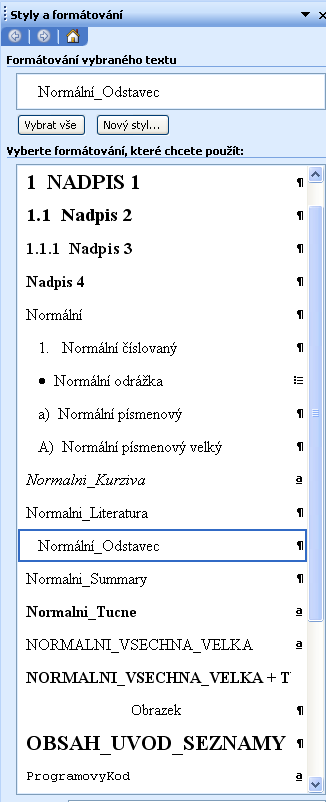
\includegraphics[width=0.2\textwidth]{./obrazky/obrazek_1.png}
      \caption {Styly (převzato z: \cite{Celikyilmaz2009})}
      \label{fig:44}
    \end{figure}

    %ukázka odkazu na zkratky a obrázek
    \Gls{GIT} \Gls{CAD} bla bla bla \odkazObrazek{fig:44}. Pokud chceme uvést překlad z angličtiny můžeme to udělat takto \transl{english words}.

    %dají se dělat i složené obrázky
    \begin{figure}
        \centering
        \begin{subfigure}[b]{0.45\textwidth}
          \centering
          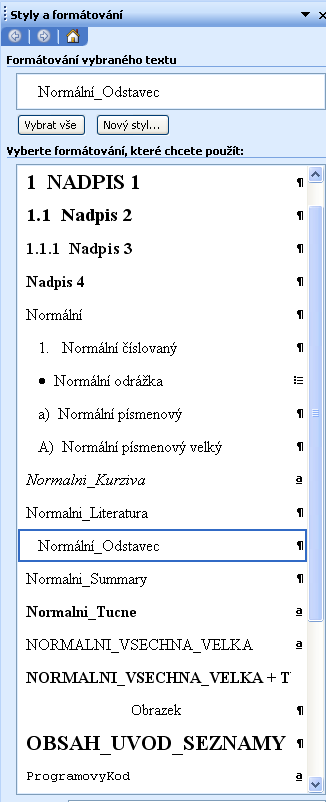
\includegraphics[width=\textwidth]{./obrazky/obrazek_1.png}
          \caption{Cena za metr čtvereční bytů v Londýně (převzato z:\cite{Fotheringham2002})}
          \label{fig2.1}
        \end{subfigure}%
        \quad %add desired spacing between images, e. g. ~, \quad, \qquad etc.
          %(or a blank line to force the subfigure onto a new line)
        \begin{subfigure}[b]{0.45\textwidth}
          \centering
          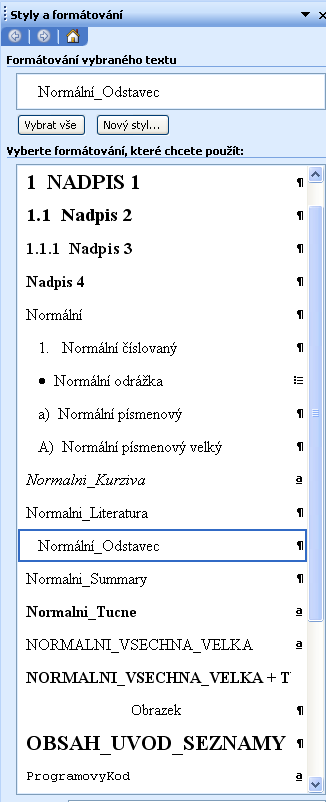
\includegraphics[width=\textwidth]{./obrazky/obrazek_1.png}
          \caption{Obsah zinku v půdě (převzato z:\cite{Hengl2009})}
          \label{fig2.2}
        \end{subfigure}
        \caption{Povrch socioekonomického (a) a fyzickogeografického (b) ukazatele}
        \label{fig2}
    \end{figure}

    \begin{table}[h]
    \caption {Ukázková tabulka}
    \label{tab1}
    \centering
      \begin{tabular}{ |l|l|l| }
        \hline
        \multicolumn{3}{ |c| }{Team sheet} \\
        \hline
        Goalkeeper & GK & Paul Robinson \\ \hline
        \multirow{4}{*}{Defenders} & LB & Lucus Radebe \\
        & DC & Michael Duberry \\
        & DC & Dominic Matteo \\
        & RB & Didier Domi \\ \hline
        \multirow{3}{*}{Midfielders} & MC & David Batty \\
        & MC & Eirik Bakke \\
        & MC & Jody Morris \\ \hline
        Forward & FW & Jamie McMaster \\ \hline
        \multirow{2}{*}{Strikers} & ST & Alan Smith \\
        & ST & Mark Viduka \\
        \hline
      \end{tabular}
    \end{table}

    Odkaz na tabulku pak vytvoříme takto: \odkazTabulka{tab1}.

    \begin{equation}
    \label{eq1}
    c = \sqrt{a^2 + b^2}
    \end{equation}

    Vzorce pak odkazujeme \odkazVzorec{eq1}. 

    Citace se dají dělat buď jako \citep{Talasova2003} nebo \cite{Talasova2003}.




    %------------------------------------------------------------------------- TEORETICKÁ VÝCHODISKA
    \newpage
    \section{TEORETICKÁ VÝCHODISKA}
      Databáze je strukturovaná kolekce dat. Slouží pro efektivní ukládání dat a jejich zpětně čtení \citep{Oppel2009}. V relační databáze jsou ukládána ve formě tabulek, tedy entit a atributů, a jsou vzájemně propojeny logickými vazbami, které se nazývájí {\it relace} \citep{Connolly2005}. Toto logické uložení vazeb mezi tabulkami umožňuje efektivní manipulaci s daty, rychlé vyhledávání i komplexní analýzu \citep{Momjian2001}. 

Základy {\it relační databáze} položil v roce 1970 matematik E. F. Codd, který relačnímu modelu přidal i srozumitelné příkazy vycházejících z běžné angličtiny, které jsou dnes známy jako jazyk {\it SQL} (Structured Query Language)\citep{Zak2001}. V dnešní době je možné setkat se také s pojmy objektová a objektově-relační databáze, které přebírají řadu vlastností z oblasti objektového programování.

Obvykle se rozlišují pojmy databáze, který odkazuje na obecný koncept, a pojem databázový systém nebo přesněji {\it systém řízení báze dat} \footnote{angl. Database Management System (DBMS)}, což je konkrétním počítačovým program, který zajišťuje fyzické uložení dat. Moderní SŘBD jsou navrženy na principu klient/server, kdy databáze běží jako služba na pozadí a čeká na dotazy od klientů. Server umožňuje uživatelům přístup k databázi, vytváření a aktualizace dat, stejně jak jako vyhledávání či analýzu \citep{Connolly2005}. Uživatel s databázi komunikuje skrze jazyk SQL většinou v kombinaci s vlastním jazykem daného databázového systému.

Pro uložení dat malého projektu je samozřejmě možno použít i jiného formátu určeného pro ukládání dat, například soubory formátu XLS, XML, CSV či moderního JSON. Pro komplexní správu dat velkého projektu je však databáze pro své relace více než vhodná. 

Prostorová databáze, někdy také zvaná geodatabáze, není nic jiného než databáze obohacená o datový typ určený pro ukládání prostorové informace o prvku, prostorové indexy a sadu funkcí vhodných pro správu prostorových dat. Více informací o prostorových databázích viz kapitola \odkazKapitola{PostgreSQL} PostgreSQL 9.x (PostGIS) a \odkazKapitola{MSSQL} MS SQL Server 2008. 

Prostorová data, také zvaná geodata, jsou z pohledu společnosti Esri prvky, které nesou informaci o geografické poloze, zakódovanou informaci o tvaru (bod, line, polygon) a popis geografického jevu. Tato geodata jsou uložená ve formátu, který je možno použít v geografickém informačním systému \citep{Esri2006}. Příkladem takového formátu může být vektorový Esri shapefile, Esri coverage, GML, KML, GeoJSON nebo rastrový Erdas Image a GeoTIFF. Dalším způsobem je již zmíněná databáze, do níž se vektorová data ukládají ve specifickém tvaru daném standardem OGC\footnote{OGC standardy jsou kontrolované konsorciem Open Geospatial Consortium,\newline zdroj \url{http://www.opengeospatial.org/ogc}} Simply Feature for SQL 1.2.1, který specifikuje způsob uložení dat v digitální podobě. Simply Feature je založen na 2D geometrii s~možností lineární interpolace mezi lomovými body. To umožňuje vložení následujících prvků:

        \begin{itemize}
          \item bod - POINT(0 0),
          \item linie - LINESTRING(0 0, 1 1, 1 2),
          \item polygon - POLYGON ((0 0,4 0,4 4,0 4,0 0),(1 1, 2 1, 2 2, 1 2,1 1)),
          \item série bodů - MULTIPOINT((0 0),(1 2)),
          \item série linií - MULTILINESTRING((0 0,1 1,1 2),(2 3,3 2,5 4)),
          \item geometrická kolekce, která může obsahovat různé geoprvky (body, linie i polygony) - GEOMETRYCOLLECTION(POINT(2 3),LINESTRING(2 3,3 4))\footnote{zdroj http://postgis.net/docs/manual-2.1/using\_postgis\_dbmanagement.html\#RefObject}.
        \end{itemize}

První slovo specifikace určuje druh prvku (point, linestring, polygon, multipoint,~...), následují v závorce vypsané souřadnice lomových bodů. Za tím ještě může následovat volitelný parametr kód souřadnicového systému.

Hodnoty lze dále vkládat přes Well-Known Binary (WKB) nebo Well-Known Text (WKT) reprezentaci. PostGIS funkce pro vkládání geometrie vypadá následovně:

        \begin{itemize}
          \item ST\_AsBinary(geometry) pro bitový zápis WKB
          \item ST\_AsText(geometry) pro WKT text
        \end{itemize}

Příklad použití formátu pro uložení linie do databáze s jedním lomovým bodem v souřadnicovém systému WGS84:

        \texttt{(LINESTRING(15.91 50.84, 17.20 49.64, 18.92 49.82), 4326)}

              \subsection{Vymezení pojmů}
Pro lepší porozumění textu této práce je potřeba definovat pojmy replikace, synchronizace a verzování, včetně popisu toho, jak jsou dané pojmy chápány v produktech ArcGIS. Je vhodné upozornit, že výše zmíněné procesy jsou v literatuře často užívány lehce odlišně. Některé zdroje pojmy replikace a synchronizace rozlišují, jiné je naopak považují za synonyma. 

Všechny dotyčné pojmy úzce souvisí se zálohováním dat, tedy kopírovaním dat mezi dvěmi a více uložišti. To, co tyto pojmy spojuje, je totiž vždy, v nějaké míře, zabránění ztráty dat, ať už chybou či fyzickým poškozením disku. Dané pojmy se poté liší například konkrétním způsobem provedení zálohy, či konkrétním důvodem pro použití daného procesu.

Synchronizace je obecnější pojem, který může být považován za nadmnožinou replikace. V případě, že existují dva datové zdroje, které je potřeba v daný okamžik sjednotit, je možno mluvit o synchronizaci souborů či datových složek. U souborů se shodným názvem se porovnává čas posledního zápisu, velikost nebo obsah souboru, naopak soubory, které shodu nezaznamenají, jsou jednoduše zkopírovány. Synchronizací se tedy dá proces označit v okamžiku, kdy existují nejméně dva datové zdroje a smyslem synchronizace je porovnat tato uložiště a dostat je do stejného stavu. To může například přispět snazší spolupráci více uživatelů nad stejnými daty nebo uživateli, který pracuje na více počítačích.


        %parametr H říká že to bude přímo na tom místě kde je v textu...více http://en.wikibooks.org/wiki/LaTeX/Floats,_Figures_and_Captions
          \begin{figure}[H]
            \centering
            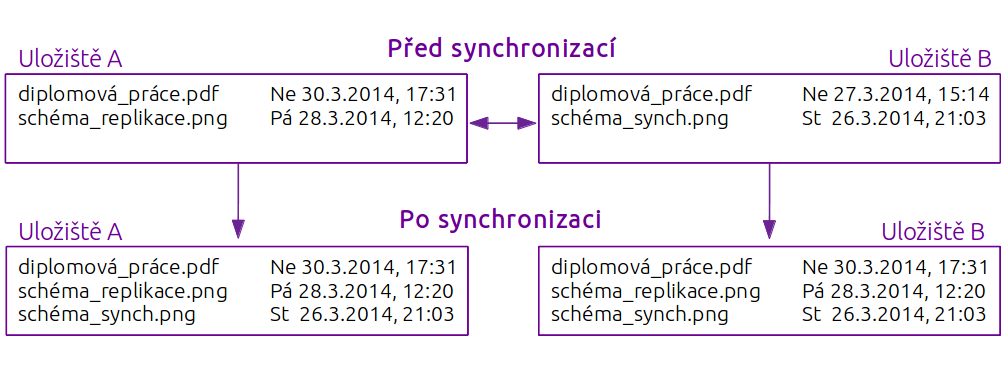
\includegraphics[scale=1]{../../../grafy/obr/schema_synchronizace_maxiTence.png}
            \caption {Příklad obousměrné synchronizace dat mezi dvěmi datovými uložišti}
          \end{figure}

Replikace naopak začíná s daty existujícími pouze na jednom uložišti. Často je tento proces používán právě ve spojitosti s databázemi, kdy je kopie dat (také replika) tvořena z důvodu snížení zátěže serveru, či ochraně dat. Replikace je tedy často vyžadována z jiných důvodů než synchronizace a pro zajištění konzistence dat používá jiných technologií. V případě, že je již kopie vytvořena, je poté možno mluvit i o synchronizaci dat, protože replika průběžně kontroluje, zda na hlavním serveru nedošlo ke změně, a pokud ano, dané změny zkopíruje. Více se replikací zabývá kapitola \odkazKapitola{kReplikace} Replikace.

Oba procesy je možno použít jednostranně, tedy kopírovat data pouze z jednoho uložiště na druhé a nikolik opačně, nebo oboustraně, kdy se datové zdroje kopírují navzájem mezi sebou.

Specifickým způsobem zálohy dat je verzování, kdy se data na záložním datovém uložišti nepřepisují, ale systematicky ukládající v takzvaných verzích tak, aby se uživatel mohl snadno kdykoliv vrátit k předchozím stavům souborů. Smyslem verzování je zachovat všechny zvolené stavy práce, čímž se verzování liší od zálohování, kde stačí mít aktuální kopii daných dat. To, co je zde popsáno jako verzování, se v produktech ArcGIS nazývá archivování dat \citep{Law2008}. 

Verzování může probíhat ručně, poloautomatizovaně či plně automatizovaně díky speciálním nástrojům pro správu verzí, kterých je na internetu dostupná celá řada. Oblíbeným verzovací systémem programátorů je Git\footnote{více na http://git-scm.com/}, open-source nástroj pro správu verzí, který pomáhá při práci s malými i velkými projekty a podporuje týmovou spolupráci. Umožňuje vrátit jednotlivé soubory nebo celý projekt do předchozího stavu, porovnávat změny provedené v průběhu času, zjistit, kdo naposledy upravil něco, co nyní možná způsobuje problémy, kdo vložil jakou verzi a mnoho dalšího \citep{Chacon2009}. Git je vhodný zejména pro textové soubory, protože dokáže analyzovat části textu, či programového kódu a zvýraznit místa, která se změnila.
        
          \begin{figure}[H]
            \centering
            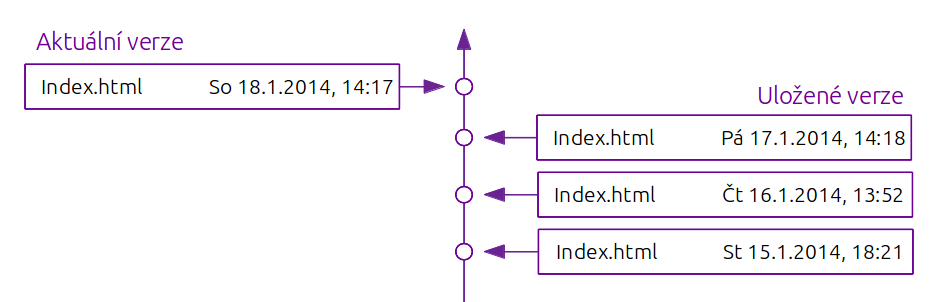
\includegraphics[scale=1]{../../../grafy/obr/schema_verzovani_maxiTence.png}
            \caption {Příklad verzování souboru}
          \end{figure}

Samotná databáze verzování dat neumožňuje. Nejsnazší způsob, jak získat verzi dat, je skriptem \texttt{dump}, který exportuje databázi do souboru. V MS SQL Serveru je tento proces nazýván Snapshot, tedy snímek databáze nebo také snímková replikace. Takový soubor se poté může verzovat podobným způsobem jako jakýkoliv jiný binární soubor typu shapefile. A to samé platí i pokud v databázi ukládáme geodata. 

Proto byl vytvořen verzovací systém také pro prostorová data, který vychází ze systému Git a nese název GeoGIT. Umožňuje uživatelům uchovávat změny v souborech shapefile, SpatialLite a z databáze PostGIS (PostgreSQL), stejně tak jako vrátit se k jakékoliv z předchozích verzí. 

Verzování může být chápáno také jako vytvoření pracovní verze. V případě, že programový kód či data jsou plně funkční či správná, ale je potřeba je aktualizovat, testovat či jinak měnit, pak je vhodné vytvořit tzn. pracovní verzi, aby nedošlo k poškození té aktuální. Jedná se o kopii aktuálního stavu, na které je možno pracovat a zkoušet. V případě, že práce nedopadne podle představ, je možno změny zahodit, pokud je tomu naopak, je možno pracovní verzi sjednotit s platnou verzí. Tento způsob verzování umožňuje Git i GeoGIT a takto chápe pojem verzování i společnosti Esri.

          \begin{figure}[H]
            \centering
            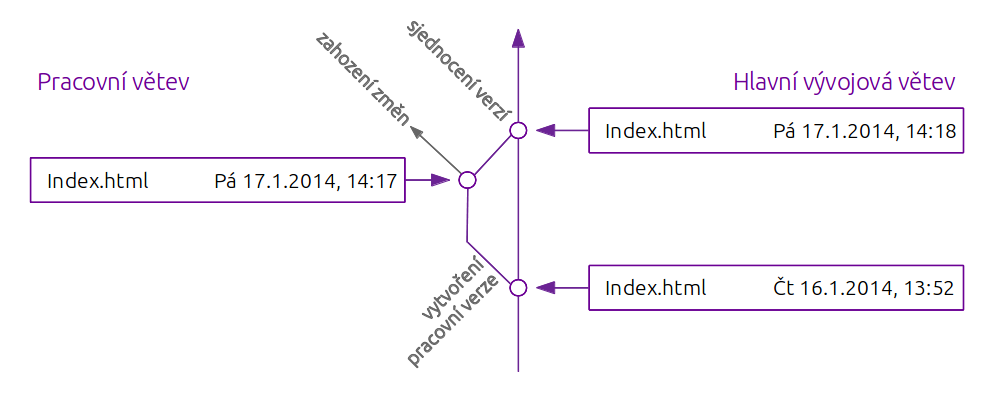
\includegraphics[scale=1]{../../../grafy/obr/schema_verzovaniBranch.png}
            \caption {Příklad verzování souboru s použitím pracovní větve}
          \end{figure}

        


              \subsection{Replikace}
        \label{kReplikace}
Replikace je proces, u kterého jsou data a databázové objekty kopírovány z jednoho databázového serveru na druhý a poté synchronizovány pro zachování souladu obou databází. Synchronizací v tomto případě myslíme kopírování všech změn, které v databázi nastanou. Použitím databáze je možno data distribuovat na různě vzdálená místa nebo mezi mobilní uživatele v rámci počítačové sítě a internetu \citep{Microsoft2013}.

Mnohé moderní aplikace se musí zabývat velkým počtem současných přístupů do databáze, což může v některých případech způsobovat problémy. Buď je server přetížen počtem připojení a data tedy přicházejí k uživateli pomalu, nebo dokonce úplně vypadne. 

Mezi časté důvody použití databázové replikace tedy patří zajištění dostupnosti dat\footnote{angl. High Availability}, resp. snížení pravděpodobnosti, že data nebudou dostupná, což může být způsobeno již zmíněným výpadkem serveru nebo například fyzickou ztrátou dat \citep{ObeHsu2012}. Další důvodem je rozložení zátěže přístupů do databáze mezi více serverů, takže nebude docházet ke zpomalení výkonu hlavního serveru ani k situaci, že data nebudou dostupná kvůli jeho výpadku \citep{BellKindahlThalmann2010}. Databáze je často zálohovaná, například skriptem dump a i to může server zpomalit. Vhodným řešením je tedy nejdříve vytvořit kopii dat na jiný datový server a až poté proces zálohování spustit. 

Všechny databáze zapojené do procesu replikace jsou v odborné literatuře nazývané uzly, angl. node. Tyto uzly dohromady tvoří replikační cluster\footnote{volně přeloženo jako skupina serveru zapojených do replikace}. Při správně nastavené replikaci, jejímž cílem je zajištění vysoké dostupnosti dat (HA), by v clusteru nikdy neměly být méně než tři uzly. Může se totiž stát, že vypadne jeden ze dvou uzlů, čímž dojde, ikdyž jen na krátkou chvíli, k situaci, že data nebudou v daný okamžik zálohovaná. 

Uzly v replikačním clusteru mohou mít jednu ze dvou základních rolí, nejčastěji nazývaných master a slave. Master server nebo pouze master je server, který poskytuje data k replikaci, má práva na čtení i zápis a probíhají tedy na něm veškeré aktualizace. Je možno se setkat také s pojmenováním Primary server, Provider, Sender, Parent nebo Source server. Naprosto jiný pojem zavádí SQL Server, který tento zdrojový server nazývá Publisher (česky Vydavatel). Druhý databázový server je nejčastěji nazýván slave, Standby, Reciever, Child nebo Subsciber (česky Odběratel). Poslední pojem je také používán SQL Serverem. Na tento server, který je dostupný vždy jen pro čtení dat, se data a aktualizace kopírují, není však možné na něj změny zapisovat \citep{RiggsKrossing2010}.

        %parametr H říká že to bude přímo na tom místě kde je v textu...více http://en.wikibooks.org/wiki/LaTeX/Floats,_Figures_and_Captions
          \begin{figure}[H]
            \centering
            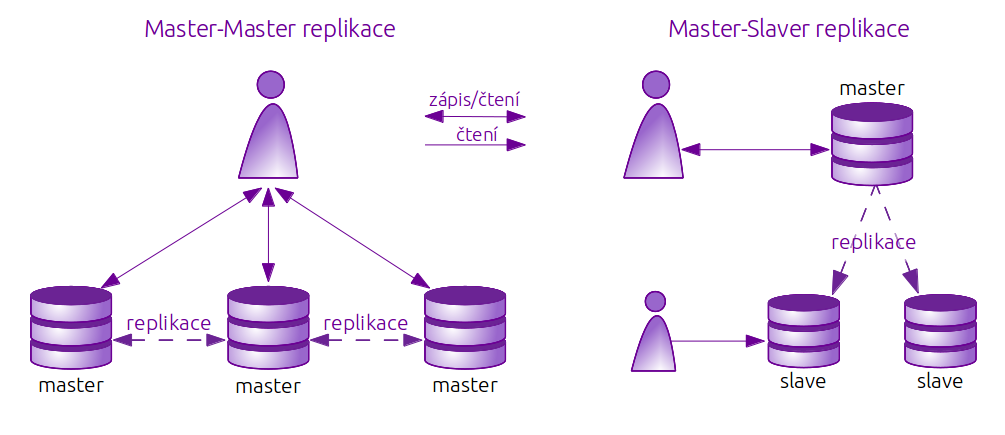
\includegraphics[scale=1]{../../../grafy/obr/schema_masterMasterSlave.png}
            \caption {Srovnání Master-Master a Master-Slave replikace}
            \label{srovnaniM-M-S}
          \end{figure}

Podle počtu master a slave serverů v replikačním clusteru, se rozlišuje zda se jedná o jednosměrnou nebo obousměrnou replikaci. Tzv. master-master replikace umožňuje zapisovat do všech uzlů v replikačním clusteru, což může být praktické například při použití databáze offline \odkazObrazek{srovnaniM-M-S}. Změny se tedy synchronizují mezi všemi databázovými uzly. Tento způsob však nese značné komplikace, je potřeba řešit konflikty změn ve stejných datech a je relativně náročný na údržbu. Tato práce se zabývá použitím druhé způsobu, tzv master-slave replikace. Tato replikace používá vždy jen jeden master server v clusteru a dva a více slave servery. Kopie dat tedy probíhá jednosměrně, vždy z master na slave servery. Podle Bella a kol. (2010) mají moderní aplikace často více čtenářů než zapisovatelů, proto je zbytečné, aby se všichni čtenáři připojovali na stejnou databázi jako zapisovatelé a zpomalovali tím jejich práci \citep{BellKindahlThalmann2010}. Z toho důvodu je tedy použití master-slave replikace více než vhodné.

Při návrhu replikace je potřeba se zamyslet také nad tím, zda bude synchronní či asynchronní. Synchronní replikace neumožní potvrzení transakce modifikující data, dokud všechny změny nejsou přeneseny na slave server \citep{Boszormenyi2013}. Tento přístup zajistí, že žádná data nebudou v průběhu transakce ztracena. V některých případech tento způsob může zbytečně zpomalit rychlost přístupu do databáze, protože je nutno čekat na každou nedokončenou transakci. Zároveň může způsobit snížení dostupnosti databáze, protože v případě, že se například přeruší spojení mezi servery, nemůže být na master serveru potvrzena žádná další transakce. Ale jistě si najde své opodstatění například při bankovních transakcích, kde je potřeba, aby všechny operace proběhly na obou stranách. V tomto případě je užití tohoto způsobu zcela nezbytné. 

Druhým způsobem je asynchronní replikace, při které se nová data mohou zapisovat na master server, přestože ještě nedošlo k replikaci stávajících dat na slave server \citep{ObeHsu2012}. To je sice za běžného provozu rychlejší, v některý případech však může způsobit nekonzistenci dat, například když proběhne transakce na master serveru, který však spadne dřív, než se změna zapíše na slave. V takovém případě se slave změní na master server, ale zároveň se nikdy nedozví o transakci, o které má uživatel informace, že proběhla v pořádku. 

        \begin{figure}[H]
          \centering
          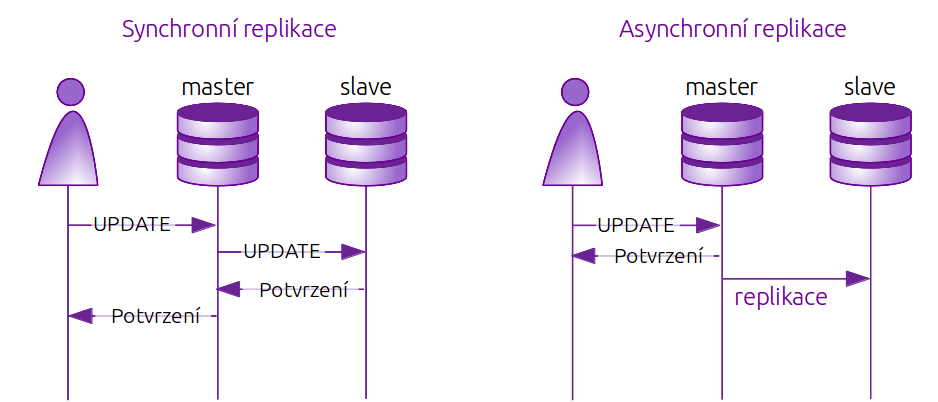
\includegraphics[scale=1]{../../../grafy/obr/schema_asyncSync_maxiTence.png}
          \caption {Rozdíl mezi synchronní a asynchronní replikací}
        \end{figure}
Replikace v PostgreSQL umožňuje plnou kopii dat z databáze i pouze výběr některých tabulek. Více o možnostech a způsobech nastavení replikace v kapitolách \odkazKapitola{kPriprava} Příprava prostředí pro konfiguraci a \odkazKapitola{kKonfigurace} Konfigurace replikace.

Dále je možno rozlišovat replikaci pole toho, zda je logická nebo fyzická. Fyzická replikace na druhý server kopíruje bloky binárních datových souborů bez znalosti jejich struktury (sloupce, řádky, …), čímž se zajistí identická replika. Pro tento způsob kopírování dat, která mají jasně danou strukturu, je potřeba mít na obou serveru stejnou platformu a architekturu. Tento způsob je velice spolehlivý a často snazší na konfiguraci. 

Naopak logická přenáší data v textové podobě, která nese informace o příkazu a struktuře. Tento způsob je více flexibilní, umožňuje výběr jen několika databází nebo tabulek a není závislý na architektuře ani operačním systému \citep{Boszormenyi2013}. 

Posledním diskutovaným pojmem je kaskádová replikace, která umožňuje připojit repliku k jinému slave serveru místo k hlavnímu master serveru. Tento způsob může být výhodných předeším z těchto dvou důvodů. Řekněme, že se kaskádová replikace použivá při existenci většího počtu slave serverů v clusteru, třeba sta. V případě, že by se všechny repliky připojovaly k hlavnímu serveru, došlo by u něj k razantnímu zpomalení jeho výkonu. Kaskádová replikace může být praktická také v okamžiku, kdy se data přenáší na velkou vzdálenost, třeba do Číny. V případě, že mají v Číně dvě repliky, je zcela zbytečné, aby se obě kopie přenášely na tak velkou vzdálenost, když druhá replika se může připojit k první a mít data s mnohem menším zpožděním.

          \begin{figure}[H]
            \centering
            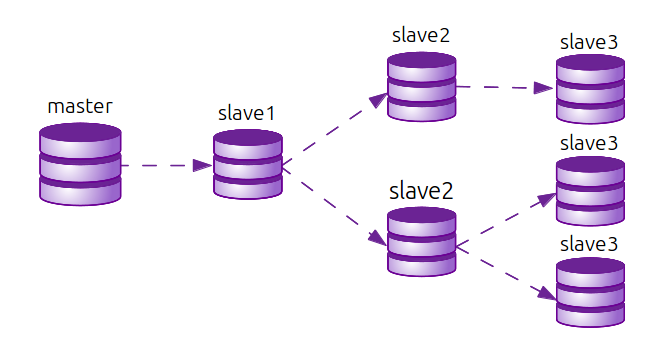
\includegraphics[scale=1]{../../../grafy/obr/schema_kaskadova.png}
            \caption{Ukázka kaskádové replikace}
            \label{kaskadova}
          \end{figure}

Každý databázový server (myšleno SŘDB) si volí terminologii a konkrétní nastavení mírně odlišně. Tato kapitola se snaží popsat chápání replikace co v největší míře obecně s ohledem na použití tohoto pojmu v PostgreSQL. Zcela jinou terminologii, ikdyž založenou na stejných principech, zavádí SQL Server, který pro export databáze do souboru používá pojem snímková replikace, pro master-slave replikaci pojem transakční replikace a pro master-master replikaci slučovací replikace. 




      
\subsection{ArcGIS produkty}

V názvu práce se objevuje spojení Esri platforma, čímž jsou chápány produkty americké společnosti Esri založené v roce 1969 manželi Dangermondovými, a zabývájící se vývojem software zaměřeného na geografické informační systémy \footnote{více informací \url{http://www.esri.com/about-esri/history}}.

Z hlediska chápání Esri má GIS tři roviny. První je to GIS jako prostorová databáze reprezentující geografické informace, dále sada map zobrazující prvky a vztahy mezi prvky na zemském povrchu a zároveň i software pro GIS jako sada nástrojů pro odvozování nových informací ze stávajících. Esri tyto tři pohledy na GIS propojuje v software ArcGIS jakožto kompletní GIS, který se skládá z katalogu (kolekce geografický datových sad), map a sad nástrojů pro geografické analýzy.

Esri vytváří integrovanou sadu softwarových produktů ArcGIS, které poskytují nástroje na kompletní správu GIS a přizpůsobují produkty různým úrovním nasazení. Výběr produktu záleží na tom, zda zákazník požaduje jedno nebo více uživatelský systém, zda se má jednat o stolní systém nebo server, popř. zda má být dostupný prostřednictvím internetu. Nabízí také produkty vhodné pro práci v terénu \citep{Esri2006}.

Základními produkty\footnote{Názvy jednotlivých produktů použitých v tomto odstavci jsou platné od verze ArcGIS 10.1. Starší verze ArcGIS používají jiné názvy, jejichž přehled je možný na stránkách firmy ARCDATA Praha \url{http://www.arcdata.cz/produkty-a-sluzby/software/arcgis/prejmenovani-arcgis/.}} jsou stolní systémy ArcGIS for Desktop ve verzích Basic, Standard, Advanced\footnote{zdroj \url{http://www.esri.com/software/arcgis/about/gis-for-me}}, dále serverové verze ArcGIS for Server (pro Linux a Windows) ve třech úrovních funkcionality (Basic, Standard, Advanced) a dvou úrovních kapacity serveru (Workgroup a Enterpise). Další produkt ArcGIS for Mobile, ve verzích ArcPad, ArcGIS for Windows Mobile a ArcGIS for Smartphone and Tablet, je určený především pro práci v terénu. A v neposlední řadě verze dostupná skrze internet ArcGIS Online. K tomu všemu Esri přidává velké množství extenzí a dalších verzí\footnote{kompletní seznam na oficiálních webových stránkách Esri \url{http://www.esri.com/products} nebo \url{http://www.arcdata.cz/produkty-a-sluzby/software/arcgis/}}.

        \begin{table}[H]
          \caption{Varianty programu ArcGIS platné od verze 10.1.}
          \label{verzeArcGIS}
          \begin{footnotesize}
            \begin{center}
              \rowcolors{1}{white}{lightgray}
              \begin{tabular}{|>{\centering} c |>{\centering}m{9.5em}  m{8.5em}  <{\centering} m{11em}  <{\centering}|}
                \hline
                {\bf \color{purpurova7}Produkt}	& \multicolumn{3}{c|}{\bf \color{purpurova7}Verze} \\
                \hline
                ArcGIS for Desktop & Basic & Standard & Advanced \\
                 ArcGIS for Server &	Basic &	Standard &	Advanced \\
                 ArcGIS for Mobile &	ArcGIS for Windows Mobile &	ArcPAD &	ArcGIS for Smartphone and Tablet \\
                   ArcGIS Online   & & &	\\	
                \hline
              \end{tabular}
            \end{center}
          \end{footnotesize}
        \end{table}

        Dle \cite{Law2008} je nativním formátem produktů ArcGIS geodatabáze a jsou rozlišovány tři druhy geodatabáze. Ani v jednom případě se však nejedná o databázi v pravém slova smyslu, tak jako ji chápame v \odkazKapitola{PostgreSQL} a \odkazKapitola{MSSQL}. V každém případě však tyto způsoby umožňují uložení, přístup a správu dat. U prvních dvou typů, personální a souborové geodatabáze, se data ukládají do jednoho binárního souboru, kde jsou však ukládaná ve stejné struktuře jako v plnohodnotném databázovém serveru. Do takového geodatabáze můžeme uložit více než jednu vrstvu, což je výrazný rozdíl oproti formátu shapefile. Výhodou je dále možnost použití relací, sofistikované dotazování a v neposlední řadě i snadná přenostitelnost, protože takováto databáze bude vždy jen jeden soubor obsahující několik vrstev. Oproti tomu shapefile, který obsahuje jen jednu vrstvu, je tvořen minimálně 4 soubory. Oba tyto typy podporují pouze jednoho editujícího uživatele a mnoho uživetelů s právem čtení. Nepodporují dlouhé transakce ani verzování.

        \begin{table}[H]
          \caption{Přehled rozdílů personální a souborové geodatabáze v ArcGIS}
          \label{verzeArcGIS}
          \begin{footnotesize}
            \centering
            \begin{center}
              \rowcolors{1}{white}{lightgray}
              \begin{tabular}{|>{\centering} m{10.2em} |>{\centering}m{10.2em}  m{10.2em}  <{\centering}|}
                \hline
                {\bf \color{purpurova7}databáze}	& {\bf \color{purpurova7}souborová .gdb\textsuperscript{1}} & {\bf \color{purpurova7}personální .mdb\textsuperscript{1}}\\
                \hline
                datové uložiště/ databázový server & lokální souborový systém &	MS Access \\
                licence & ArcGIS for Destop (všechny verze) & ArcGIS for Destop (všechny verze) \\
                operační systém & Windows (možná i jiné) & Windows \\
                požaduje ArcSDE & ne &	ne \\
                vlastní datový typ & ne &	ne \\
                víceuživatelská editace & ano, ale s limity &	ne \\
                počet editorů	&	1 pro každý dataset \newline nebo tabulku\textsuperscript{2} &	1\textsuperscript{2} \\
                počet čtenářů &	více než 1\textsuperscript{2} &	více než 1\textsuperscript{2} \\
          master server\textsuperscript{3} & ne\textsuperscript{1} &	ne\textsuperscript{1} \\
            slave server\textsuperscript{3} & ano &	ano \\
                \hline
                \multicolumn{3}{l}{\textsuperscript{1}\scriptsize{http://www.esri.com/software/arcgis/geodatabase/singlex-user-geodatabase}} \\
                \multicolumn{3}{l}{\textsuperscript{2}\scriptsize{http://help.arcgis.com/en/arcgisdesktop/10.0/help/index.html\#//003n00000007000000}} \\
                \multicolumn{3}{l}{\textsuperscript{3}\scriptsize{je možno použít jako master/slave server}} \\
              \end{tabular}
            \end{center}
          \end{footnotesize}
        \end{table}

        Tato práce se více zaměřuje na třetí typ, technologii ArcSDE, kterou v některých materiálech nazývají {\it geodatabáze ArcSDE}. Nejedná se o geodatabázi, ale spíše o zprostředkovatele komunikace mezi programem ArcGIS a databázovým server. Umožňuje víceuživatelský přístup, verzování i replikaci \citep{Esri2006}. Tato technologie využívá jako datové uložiště některý z již existujících databázových serverů, např. níže popsané PostgreSQL nebo SQL server. Touto technologií se více bude zabývat kapitola \odkazKapitola{kArcSDE} ArcSDE geodatabase.


      \subsection{Použité programové prostředky}

\subsubsection{PostgreSQL 9.x (PostGIS)}
        \label{PostgreSQL}
        PostgreSQL je objektově-relační databázový systém s otevřeným zdrojovým
        kódem dostupný na většině platforem. Je volně k dispozici pro použití,
        modifikaci a znovu rozšíření způsobem, který si sami zvolíme. Jedná se
        o robustní, výkonný, bezpečný, kompatibilní a interoperabilní software
        s podporou a dobře komentovaným zdrojovým kódem. Vyhovuje standardům
        SQL od verze SQL 2008 a nabízí velké množství pokročilých funkcí.
        PostgreSQL je založen na architektuře klient-server, to znamená, že
        server pořád běží a čeká na dotazy klienta \citep{Momjian2001}. 

        S vývojem databázového serveru PostgreSQL začala University of
        California v Berkley již více než před 20 lety. Nyní je vyvíjen a
        udržován velkou komunitou nezávislých vývojářů. Používá licenci TPL
        (The PostgreSQL Licence), která je mírně odlišná od open-source licence
        BSD (Berkeley Distribution Software), ze které vychází
        \citep{RiggsKrossing2010}

        Řadí se mezi nejpokročilejší databáze díky schopnosti pracovat s
        velkými objemy dat, díky své rychlosti a funkcionalitě může soupeřit i
        s populárními komerčními systémy jako je Oracle, IBM DB2, Microsoft SQL
        Server 2008 a dalšími \citep{PostgreSQL2012}.

        Samotné PostgreSQL neobsahuje datové typy a funkce vhodné pro správu
        prostorových dat. K tomu je nutné přidat nástavbu PostGIS, která
        rozšiřuje databázi PostgreSQL o podporu geografických dat. PostGIS
        implementuje specifikaci „Simple Features for SQL“ konsorcia OGC.
        PostGIS umožňuje ukládání geometrických objektů (bod, linie, polygon),
        použití prostorových funkcí pro určení vzdáleností, délky linií, výměr
        a obvodu ploch, výběr indexu při spojení prostorových a atributových
        dotazů a mnoho dalších.

        PostGIS používá dva základní prostorové datové typy geography a
        geometry. Typ geography ukládá souřadnice v kartézských rovinných
        souřadnicích, kterým odpovídá souřadnicový systém WGS84. Je zejména
        vhodný pro malá území. Při výpočtu vzdálenosti dvou bodů tento datový
        typ vrátí jako výsledek nejkratší vzdálenost v kilometrech v rovině.
        Typ geometry data ukládá v polárním rovinném systému a umožňuje
        nastavit souřadnicový systém podle potřeb. Výsledkem dotazu na
        vzdálenost dvou bodů tedy bude úhel ve stupních. Po převodu do metrické
        soustavy dostaneme nejkratší vzdálenost na kouli. Při výběru datového
        typu může být rozhodující například počet funkcí, kterých typ geometry
        poskytuje mnohem více než geography, nebo velikosti daného území
        \citep{OpenGeo2012}.

        Existuje také další nástavba PostGIS Raster, která rozšiřuje ukládání a
        manipulaci s rastrovými daty, nástavba PostGIS Topology pro
        topologickou správu vektorových dat a pgRouting pro síťové analýzy.
        PostGIS je podporován velkou řadou software zabývajících se správou
        geografických dat, což také umožňuje snadnou přenositelnost a
        použitelnost jednotlivých nástaveb (příklad software podporujících
        PostGIS: QGIS, GvSIG, GRASS, ArcGIS).

        PostGIS používá mnoho běžně používaných knihoven jako GEOS (Geometry
        Engine Open Source) pro implementaci jednoduchých prostorových prvků a
        metod pro topologii, PROJ4 pro převod mezi kartografickými projekcemi
        nebo GDAL/OGR (Geospatial Data Abstraction Library) pro převod mezi
        různými vektorovými i rastrovými formáty \citep{ObeHsu2011}. PostGIS
        1.5. obsahovala přes 800 funkcí, typů a prostorových indexů
        \citep{ObeHsu2012}. Aktuální verze PostGIS\footnote{Aktuálně na
        http://postgis.refractions.net/} je 2.1.

        PostgreSQL podporuje replikaci i synchronizaci bez nutnosti další
        instalace. 

        Od verze ArcGIS 9.3. je PostgreSQL oficiálně podporovanou databází pro
        ukládání geodat v produktech ArcGIS. Při instalaci je pouze potřeba
        zajistit kompatibilitu verzí. Pro verzi ArcGIS 10.1 jsou podporované
        verze PostgreSQL 9.0 a PostGIS 1.5., pro ArcGIS 10.1
        SP1\footnote{Service Pack 1} je to PostgreSQL 9.1.3 a PostGIS 2.0
        \citep{OSGEO2013}\footnote{Zdroj a další informace na stránkách
        PostgreSQL http://trac.osgeo.org/postgis/wiki/UsersWikiPostgisarcgis
      nebo ArcGIS http://resources.arcgis.com/en/help/system-requirements/10.1/index.html\#//015100000075000000}.
    Databáze PostgreSQL se dá v ArcGIS produktech použít dvojím způsobem. Buď
    jen jako uložiště dat bez přidání geografického datového typu, nebo včetně
    datového typu, tedy včetně PostGIS knihovny. ArcSDE podporuje pouze datový
    typ PostGIS Geometry a přidává vlastní datový typ Esri St\_Geometry.
    Výhodou použivání Esri St\_Geometry je nezávislost na zvoleném databázovém
    systému, tedy snazší přenostitelnost celého řešení. 

        Práce byla testována na verzích PostgreSQL\footnote{Více na
        http://www.postgresql.org/} 9.1.4 a PostGIS 2.0.

        \subsubsection{Microsoft SQL Server Express 2008}
        \label{MSSQL}
        Microsoft SQL Server (dále MS SQL Server) je relační databázový systém vyvíjený
        společností Microsoft dostupný pro různé verze operačního systému Windows.
        Dodává se v mnoha verzích, které lze nainstalovat na různé hadrwarové platformy
        na základě odlišných licenčních modelů \citep{Whalen2008}. Podle Leitera (2009)
        SQL Server nabízí 8 základních verzí: Enterprise, Standard, Workgroup, Web,
        Express, Express Advanced Edition, Developer Edition a Compact Edition.
        Enterprise edition podporuje naprosto vše, co SQL Server nabízí, naopak verze
        Express, která je dostupná zdarma, obsahuje omezení některých funkcí a proto je
        vhodná spíše pro malé nebo začínající projekty \citep{Leiter2009}.

        Prostorová data jsou implementována jako CLR rozšíření a přidávají databázovému
        serveru dva prostorové datové typy geometry a geography. Rozdíl mezi datovými
        typy je podobný jako u PostgreSQL. První jmenovaný slouží k reprezentaci dat
        (bodů, linií, polygonů) v rovině, naproti tomu datový typ geography slouží
        ukládání stejných dat na povrchu zeměkoule. Oba typy pracují ve dvou dimenzích
        (nebere se v potaz výška). Podporuje také indexování dat, index je tvořen
        standardním B stromem \citep{Cincura2009}.

        SQL Server je podporován a používán ArcGIS produkty od začátku jeho vývoje.
        Verze ArcGIS Enterprise může být propojena s jakoukoliv uživatelem zvolenou a
        zakoupenou licencí databázového systému. Verze ArcSDE Desktop a Workgroup
        používají verzi Express, která je dostupná zdarma a podporuje většinu
        základních funkcí. Replikaci plně podporuje verze Enterprise, ostatní verze ji
        podporují pouze s omezenými funkcemi. Avšak již zmiňovaná verze Express, která
        je podporávána ArcSDE Desktop a Workgrorp, může být použita pouze slave server,
        tedy odběratelem replikovaných dat, není tedy možné do takovéto databáze
        připojené do replikačního clusteru zapisovat. Nemůže být tím, kdo poskytuje
        data k replikaci \citep{Whalen2008}. Stejně jako u PostgreSQL platí, že si
        uživatel může zvolit, zda použije datový typ, který je součastí ArcSDE, nebo
        ten, který je implementován do SQL Serveru. 

        \subsubsection{ArcSDE geodatabase}
        \label{ArcSDE}
        ArcSDE je technologie firmy Esri pro správu geoprostorových dat uložených v
        relačních databázových systémem. Jedná se o otevřenou a interoperabilní
        technologii, která podporuje čtení a zápis mnoha standardů. Využívá jako své
        nativní datové struktury standard konsorcia OGC Simple Feature a prostorový typ
        ISO pro databázové systémy Oracle, IBM DB2 a Informix. Poskytuje vysoký výkon a
        je přizpůsobena velkému počtu uživatelů \citep{Esri2006}.

        ArcSDE je prostředník pro komunikaci mezi klientem (př. ArcView) a SQL databází
        (př. PostgreSQL). Umožňuje přístup a správu dat v databázi, současnou editaci
        jedné databáze více uživateli, zajišťuje prostorový datový typ (St\_Geometry),
        dále integritu dat, dlouhé transakce a práci s verzemi \citep{Law2008}.

        Technologie ArcSDE vyžaduje dvě úrovně: databázovou a aplikační, která se
        skládá z ArcObjects a ArcSDE. Databázová úroveň zajišťuje jednoduchý, formální
        model pro uložení a správu dat ve formě tabulek, definici typů atributů
        (datových typů), zpracování dotazů či víceuživatelské transakce
        \citep{Law2008}. ArcSDE podporuje databázové systémy IBM DB2, IMB Informix,
        Oracle, Microsoft SQL, PostgreSQL \citep{Esri2013a}.

        Existují tři úrovně ArcSDE databáze: desktop (ArcSDE Desktop), skupinová
        (ArcSDE Workgroup) a podniková (ArcSDE Enterprise). Každá verze má jiné
        parametry a umožňuje různou úroveň editace \odkazTabulka{sde}. 

        \begin{table}[H]
          \caption[Přehled verzí ArcSDE, jejich parametrů a možností]{Přehled verzí ArcSDE, jejich parametrů a možností}
            \label{sde}
          \begin{footnotesize}
            \begin{center}
              \rowcolors{3}{lightgray}{white}
              \begin{tabular}{|>{\centering} m{9.5em} |>{\centering} m{9.5em} >{\centering} m{9.5em} m{9.5em}  <{\centering}|}
                \hline
                \multirow{2}{*}{{\bf \color{purpurova7}databáze}} & \multicolumn{3}{c|}{\bf \color{purpurova7}ArcSDE} \\
                & {\bf \color{purpurova7}Desktop\textsuperscript{1}} & {\bf \color{purpurova7}Workgroup\textsuperscript{1}} & {\bf \color{purpurova7}Enterprise\textsuperscript{1}}\\
                \hline
                  databázový server & SQL Server Express & SQL Server Express &	PostgreSQL, Oracle, SQL Server a další \\
                              licence & ArcGIS for Destop &	ArcGIS for Server Workgroup	& ArcGIS for Server Enterprise \\
                   operační systém & Windows & Windows & multiplatformní \\
                     požaduje ArcSDE & ano & ano & ano \\
                 vlastní datový typ & ne & ne & ano \\
           víceuživatelská editace & ne & ano & ano \\
                      počet editorů	&	1 &	10 & bez limitu \\
                   počet čtenářů & 3 & 10 &	bez limitu \\
                        master server\textsuperscript{2}  & ne & ne & ano \\
                         slave server\textsuperscript{2}  &	ano &	ano & ano \\
                          verzování & ano & ano & ano \\
               závislost na sítích & lokální síť & lokální síť, internet & lokální síť, internet \\
                   velikostní limity & 10GB & 10GB & záleží na velikosti serveru \\
               \hline
               \multicolumn{4}{l}{\textsuperscript{1}\scriptsize{ http://www.esri.com/software/arcgis/geodatabase/multi-user-geodatabase}}\\
               \multicolumn{4}{l}{\textsuperscript{2}\scriptsize{je možno použít jako master/slave server}} \\
              \end{tabular}
            \end{center}
          \end{footnotesize}
        \end{table}

        ArcGIS 9.2 je ArcSDE Desktop spolu s databázovým systémem MS SQL Server Express
        součástí licence produktů ArcGIS for Desktop Standard a Advanced. Takovou
        databázi mohou současně používat 4 uživatelé, z toho jen jeden může databázi
        editovat, jsou však omezeni velikostí databáze.

        Součastí licence ArcGIS for Server Workgroup je ArcSDE Workgroup, která se liší
        od verze Desktop především tím, že počet uživatelů, kteří mohou součastně
        editovat nebo prohlížet databázi, je zvýšen na deset.

        Nejvyšší úroveň, ArcSDE Enterprise, je možno získat s licencí ArcGIS for Server
        Enterprise, která uživatelům přináší nejméně omezení. Mohou si vybrat z
        několika komerčních i nekomerčních databázových systémů, počet uživatelů není
        omezen, stejně jako velikost databáze.

        K ArcSDE a vybrané databázi je možno přistupovat přes ArcCatalog, není tedy
        potřeba instalace dalšího software nebo zkušenost s administrací databáze
        \citep{Esri2006}.

        Replikaci a synchronizaci dat umožňují pouze ArcSDE Enterprise a Workgroup
        \citep{Esri2013b}. Jak už bylo zmíněno v předchozí kapitole \odkazKapitola{MSSQL} Microsoft SQL
        Server Express 2008, SQL Server Express je možný použít v replikačním clusteru
        pouze jako slave server. Vzhledem k tomu, že proces replikace je implementován
        pří do ArcObjects a ArcSDE, nezáleží na konkrétním databázovém systému
        \citep{Law2008}.



            \subsection{Nástroje pro replikaci v PostgreSQL}

      PostgreSQL nabízí hned několik nástrojů pro replikaci. Je možno použít zabudovanou streaming replikaci, která je dostupná od verze PostgreSQL 9.0, nebo některou z extenzí, například Slony-I, pgpool, Londiste, Bucardo nebo Postgres-XC, pro jejichž srovnání \vizTabulka{tSrovnaniReplikace}. Tato kapitola se dále bude zabývat nativní streaming replikací a extenzemi Slony-I a pgpool.

        \begin{table}[H]
          \caption{Srovnání různých typů dostupných replikačních řešení}
          \label{tSrovnaniReplikace}
          \begin{footnotesize}
            \begin{center}
              \rowcolors{1}{white}{lightgray}
              \begin{tabular}{|c|cccccc|}
                \hline
                {\bf \color{purpurova7}nástroje}	& {\bf \color{purpurova7}typ} & {\bf \color{purpurova7}technika} & {\bf \color{purpurova7}M/M} & {\bf \color{purpurova7}M/S} & {\bf \color{purpurova7}sync} & {\bf \color{purpurova7}async} \\
                \hline
                PostgreSQL 9.3* & fyzická & xlog     & ne  & ano & ano & ano \\ 
                      pgpool-II & logická & proxy    & ano & ne  & ano & ne  \\
                        slony-I & logická & triggers & ne  & ano & ne  & ano \\ 
                       Londiste & logická & triggers & ne  & ano & ne  & ano \\ 
                        Bucardo & logická & triggers & ano & ano & ne  & ano \\ 
                    Postgres-XC & cluster & -        & ano & ne  & ne  & ano \\ 
                \hline
                \multicolumn{3}{l}{\scriptsize{*streaming replikace}} & \multicolumn{4}{r}{\scriptsize{zdroj: Tomáš Vondra, 2011}}\\
              \end{tabular}
            \end{center}
          \end{footnotesize}
        \end{table}

      \subsubsection{Slony-I}
      \label{kSlony}

      Jak píší \cite{Boszormenyi2013} je Slony-I jeden z nejrozšířenějších externích nástrojů pro replikaci PostgreSQL databází. Zároveň se také řadí mezi nejstarší, plně používán je v PostgreSQL již od verze 7.3. a je velmi dobře podporován i dalšími externími řešeními pro PostgreSQL, například programem PgAdmin3, který nabízí správu dat pomocí grafického rozhraní \citep{Boszormenyi2013}.

      Jedná se o {\it trigger-based} replikaci, což znamená, že je ke každé tabulce vybrané pro replikaci přidán trigger, který zajistí replikaci každé změny, která v tabulce nastane. Z toho také vyplývá, že se jedná o logickou replikaci, kdy je možné replikovat pouze změny v datech, tedy tzv. DML\footnote{Data Manipulation Language} příkazy (INSERT, UPDATE, DELETE), nikoli změny struktury databáze, tedy tzv. DDL\footnote{Data Definition Language} příkazy (CREATE, ALTER, DROP). Každá změna struktury se tedy musí provést ručně, což se může jevit jako nevýhodné. Nese to ale i své klady, například možnost výběru pouze některých tabulek. Uživatel vytváří tzv. {\it replikační set}, do kterého se zapíší pouze ty tabulky, které je potřeba replikovat. 

Další výhodou, a to zvlášť v porování se streaming replikací, je možnost replikace dat mezi různými verzemi PostgreSQL bez ohledu na platformu a architekturu. Naopak spíše za nevýhodu je považováno, že si vytváři ke každé tabulce vlastní schéma, do kterého se ukládají replikovaná data, což způsobuje redundanci dat. 

  Slony-I umožňuje multimaster i master-slave replikaci, která je z principu asynchronní. 
  Slony-I replikaci je možno nastavit jako kaskádovou i jako Hot Standby, což
  znamená, že v případě pádu master serveru je slave automaticky povýšen na
  master. Slony-I má vlastní konfigurační nástroj a samotná replikace funguje
  díky vlastnímu replikačnímu démonu, který běží stále, registruje změny a
  kopíruje je na slave servery.

  \subsubsection{Streaming replikace}
  \label{kStreamingTeorie}

  Streaming replikace je nativní řešení PostgreSQL implementované od verze
  9.0. Jedná se o fyzickou replikaci, proto je nutné použití stejné verze
  PostgreSQL, stejné platformy i architektury na všech uzlech replikačního
  clusteru. 
  
  Jde se o {\it log-shipping} replikaci, což znamená, že jsou na slave servery
  posílány záznamy transakčního logu, v PostgreSQL nazývané WAL (Write Ahead
  Log). Do něj jsou změny nejdříve zaznamenávány přímým zápisem na disk a až
  poté potvzeny jako úspěšné. Tento způsob zajišťuje datům naprosté bezpečí,
  protože kdyby došlo k chybě a změny se nezapisovaly na disk, ale pouze do
  cache, mohlo by dojít k jejich ztrátě. Existuje pouze jeden transakční log
  pro jednu instalaci PostgreSQL, proto se replikují vždy všechny databáze a
  není možné výběru jen několika tabulek, tak jako u Slony-I \citep{Boszormenyi2013}. 
 
  Výhodou tohoto nativního řešení je větší efektivita a stabilita replikace,
  než nabízí jiná diskutovaná řešení. Použití toho způsobu replikace však má i
  tu nevýhodu, že aktualizaci databázového systému, operačního systému i
  architektury je třeba provést vždy na všech serverech zároveň.

  Streaming replikace umožňuje pouze master-slave replikaci ve variantách
  synchronní, asynchronní a kaskádová\footnote{podporovaná od verze PostgreSQL
  9.2} a Hot Standby mód.

      \subsubsection{pgpool}
      \label{kpgpool}

Nástroj pgpool, který je stejně jako Slony-I extenzí pro PostgreSQL, je dalším
z nástrojů, který je možno použít pro replikaci dat. Umožňuje však i další
pokročilé funkce jakými jsou sdílení spojení klienta s databází mezi servery
(angl. connection pooling), paralelní uložení dat (angl. parallel query) a
rozložení zátěže mezi více servery (angl. load balancing). 

Nástroj pgpool umožňuje sdílení spojení klienta s databází, což v praxi
znamená, že se vytvoří několik spojení se serverem, která i po skončení dotazu
zůstanou otevřená a připravená pro další použití. Nemusí se tedy navazovat
spojení při každém požadavku ze strany klienta, což velice zrychlí provoz a
zajistí plynulost užívání databáze. Je vhodným nástrojem pro správu velkých
tabulek díky distribuovanému způsobu ukládání dat \citep{pgpool2014}. 

Zároveň pgpool umožňuje rozložení zátěže mezi více serverů v replikačním
clusteru, aby nedocházelo k přetížení jednotlivých uzlů a celkově se zvýšila
rychlost a~efektivita práce s databází. V tomto se pgpool stává prostředníkem
pro komunikaci mezi klientem a serverem. 

Aby nebylo potřeba dát každému
uživateli přístup k jinému slave serveru, nebo přístupy do databáze manuálně
rozkládat skrze složité programové řešení, nabízí se možnost použití pgpool. 
Ten se navenek jeví jako jakákoliv jiný databázový server, do kterého se
uživatelé připojí a  pgpool pak sám rozdělí dotazy mezi uzly v replikačním
clusteru dle aktuální zátěže \citep{Boszormenyi2013}. Zároveň, pokud má
uživatel práva ke čtení i k zápisu, umí na základě aktuálního SQL příkazu
rozhodnout, zda jej přepošle master nebo slave serveru \odkazObrazek{opgpool}. 

Na základě vybraných funkcí je možno použít jeden ze čtyř základních módů, které pgpool poskytuje\footnote{kompletní přehled na \url{http://www.pgpool.net/docs/latest/pgpool-en.html\#config}}: základní, replikační, master/slave a paralelní. V návrh databázového řešení byl použit mód master/slave, který je dále popisován v kapitole \odkazKapitola{kpgpool}.

      \begin{figure}[H]
        \centering
        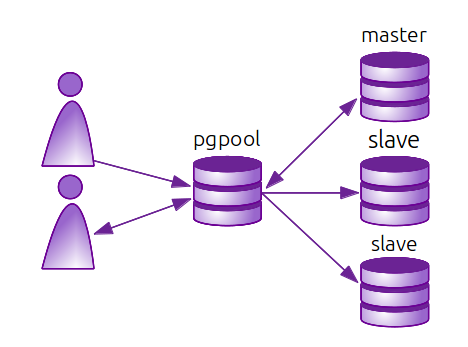
\includegraphics[scale=1]{../../../grafy/obr/schema_pgpool.png}
        \caption{Zjednodušené schéma pgpool v módu master/slave}
        \label{opgpool}
      \end{figure}



    %------------------------------------------------------------------------- VÝSLEDKY
    \newpage
    \section{NÁVRH A KONFIGURACE REPLIKACE}
      Tato kapitola se zabývá hodnocením současného stavu správy dat na katedře geoinformatiky, návrhem databázového řešení dle požadavků a možností katedry a podrobně popisuje vytvoření testovacího prostředí na serverech katedry dle vytvořeného návrhu. Do hloubky popisuje konfiguraci vybraných nástrojů, včetně jejich nasazení.

Katedra má zájem využít potenciál databázového řešení, které bude zajišťovat efektivní uložení, sdílení a správu dat, která má katedra k dispozici. Zároveň má v~plánu vyučovat problematiku správy dat v~databázi. Studenti se budou moci nejen dozvědět o způsobech uložení dat, ale také je prakticky vyzkoušet, pochopit jejich fungování, naučit se pracovat s daty nahranými do GIS software a v neposlední řadě tato data použít pro své projekty a závěrečné práce. Velkou výhodou bude také větší připravenost do praxe, kde je databázové ukládání dat hojně rozšířeno. Data uložená v~databázi pak budou mnohem snáze využitelná jak pracovníky katedry, tak i jejími studenty. 

\subsection{Aktuální stav správy dat}
\label{kAktualniStav}

Katedra aktuálně provozuje tři servery, konkrétně \texttt{virtus.upol.cz}, \texttt{atlas.upol.cz} a~\texttt{geo\-hydro.upol.cz}. Poslední z jmenovaných byl poskytnut jako testovací server pro tuto práci a v budoucnu se s ním počítá jako s master serverem pro zde popisované databázové řešení. První dva zmíněné servery jsou aktivně používány, hostují například geoportál publikovaný skrze ArcGIS Server, který je důležitým prostředkem pro prezentaci projektů a dat, která na katedře vznikají. Data ke geoportálu i dalším aplikacím běžícím na těchto serverech jsou ukládána do MS SQL Serveru, přičemž každý ze serverů obsahuje jiné datové sady, které nejsou pravidelně zálohovány, protože jejich aktualizace není příliš častá. Aktuální řešení nepoužívá replikaci dat, data tedy mohou být nedostupná z důvodu výpadku serveru. 

Databáze aktuálně obsahují data například z projektů BotanGIS\footnote{\url{http://botangis.upol.cz/botangis/mapa}}, Virtuální studovna CHKO Litovelské Pomoraví\footnote{\url{http://virtus.upol.cz/}}, dále data metadatového systému Micka\footnote{\url{gislib.upol.cz/metadata}}, data ze senzorové sítě KGI, data ke studentským pracím a také ukázková data určená pro výuku. Je založeno přibližně 10 účtů, které mají přístup pro zápis, a řádově v desítkách účtů s právem čtení, do databází aktuálně není příliš často zapisováno. 

Velké množství dat, které má katedra k dispozici, je však stále uloženo ve formátech Shapefile nebo File Geodatabase. Každý kdo chce tato data použít, musí je přenést přes různá hardwarová zařízení nebo je zkopírovat po síti. Studenti si musejí dělat kopie dat při každém cvičení, což velice zdržuje výuku. Často se totiž jedná o velké objemy dat, jejichž kopie může trvat řádově v jednotkách až desítkách minut. Data jsou poté fyzicky uložena na počítačích v učebnách, což mimo jiné dovoluje, aby se k datům dostal kdokoliv, kdo má na učebnu přístup. Není tedy přehled o tom, kdo data využívá. Studenti navíc netuší, s jakými daty pracují a nabývají nesprávných představ o tom, že všechna data jsou vždy uložená ve formátu Shapefile. Zároveň se špatně zajišťuje aktualizace dat, při které, není-li spravována centralizovaně, může docházet k nekonzistenci dat. Při kopírováním dat na různá datová uložiště je navíc těžké dodržet licenční podmínky, se kterými jsou data pořizována. 

\subsection{Požadavky na databázové řešení}
\label{kPozadavky}

Základním požadavkem byl výběr takového databázového systému, který je široce používán v oblasti geoinformatiky a zároveň je podporován produkty ArcGIS. Požadavem bylo také zhodnocení finanční stránky, replikace je totiž v mnohých komerčních systémech zařazena až mezi nejpokročilejší funkcionalitu a tedy je dostupná až s drazšími licencemi. 

Katedra má v zájmu ukládat do databáze mnohem více datových sad, které má k dispozici a které jsou momentálně dostupné pouze ve formátech Shapefile nebo File Geodatabase. Jedná se například o datové sady ArcČR500 verze 2.0 a 3.0, Data200 (ČUZK), CEDA ČR 150, data, která byla uvolněna jako podpora pro Krajinotvorný program MŽP, nebo data dostupná k produktům Esri nebo Idrisi. Databázové řešení by tedy mělo být navrženo tak, aby uneslo mnohem větší počet připojení a dotazů než v současné době, protože datového sady, které budou nově dostupné skrze databázi, budou používány v řadě cvičení. Plánem je v rámci cvičení studentům umožňit plnohodnotnou práci s daty, tedy povolit jim jak čtení dat, tak zápis do databáze. 

Návrh by měl také zohlednit zájem katedry o využití jednoho ze serverů jako slave server pro replikaci dat ze senzorové sítě Ekodata. 


      \section{Návrh replikačního řešení}
  Po provedení rešerše a zohlednění všech podmínek, požadavků a možností
  katedry, byl sestaven návrh kompletního databázového řešení založeného na
  procesu replikace. Z databázových serverů byl vybrán server PostgreSQL hned
  z~několika důvodů. Jedná se o plnohodnotný databázový systém dostupný zda\-rma
  se všemi nástroji, je široce používaný v oblasti geoinformačních technologií,
  je multiplatfomní a od verze ArcGIS 9.3 plně podporováný produkty ArcGIS.
  Návrh počítá s použitím ArcSDE pro propojení databáze s ArcGIS produkty. Při
  výběru verzí je nutné zajistit kompatibilitu verzí jednotlivých software,
  a~poté ArcSDE nainstalovat společně s PostrgreSQL.

  Byl navržen replikační cluster s nejméně třemi servery z důvodů, které již
  byly diskutovány v kapitole \ref{kReplikace}. Celý cluster poběží na stejné
  platformě a proto bude možno použít streaming replikaci se všemi výhodami
  zmíněnými v kapitole \ref{kReplikace}. Byla zvolena jednosměrná master-slave
  replikace, cluster tedy bude obsahovat jeden master a dva (popř. více) slave
  serverů. Aby nedošlo ke ztrátě dat v~případě, že by master server spadl dřív,
  než se data zkopírují na slave server, pro první slave (\texttt{slave1}) byla
  zvolena varianta synchronní replikace. Je vhodné, aby servery běžely
  v~lokální síti z důvodu rychlosti a spolehlivosti spojení mezi master a slave
  serverem. 


  Druhý server (\texttt{slave2}) bude replikovat asynchronně a zároveň, aby
  ne\-do\-chá\-ze\-lo k~přetížení master serveru, bude replikace probíhat ze
  \texttt{slave1} na \texttt{slave2}, tedy kaskádově. Tím bude řešení zároveň
  přípraveno na výpadek master serveru, protože v~případě, že master vypadne,
  \texttt{slave1} bude povýšen na master a \texttt{slave2} bude ihned moci
  replikovat. Ze \texttt{slave2} lze dále tvořit pravidelnou, například denní
  nebo týdenní, zálohu pomocí ulitily \texttt{pg\_dump}. Záloha pomocí
  \texttt{pg\_dump} tak nebude zatěžovat master server a sama o sobě bude
  probíhat rychleji, než by tomu bylo na master serveru, který je již tak velmi
  vytížen dalšími procesy.

  \begin{center}
    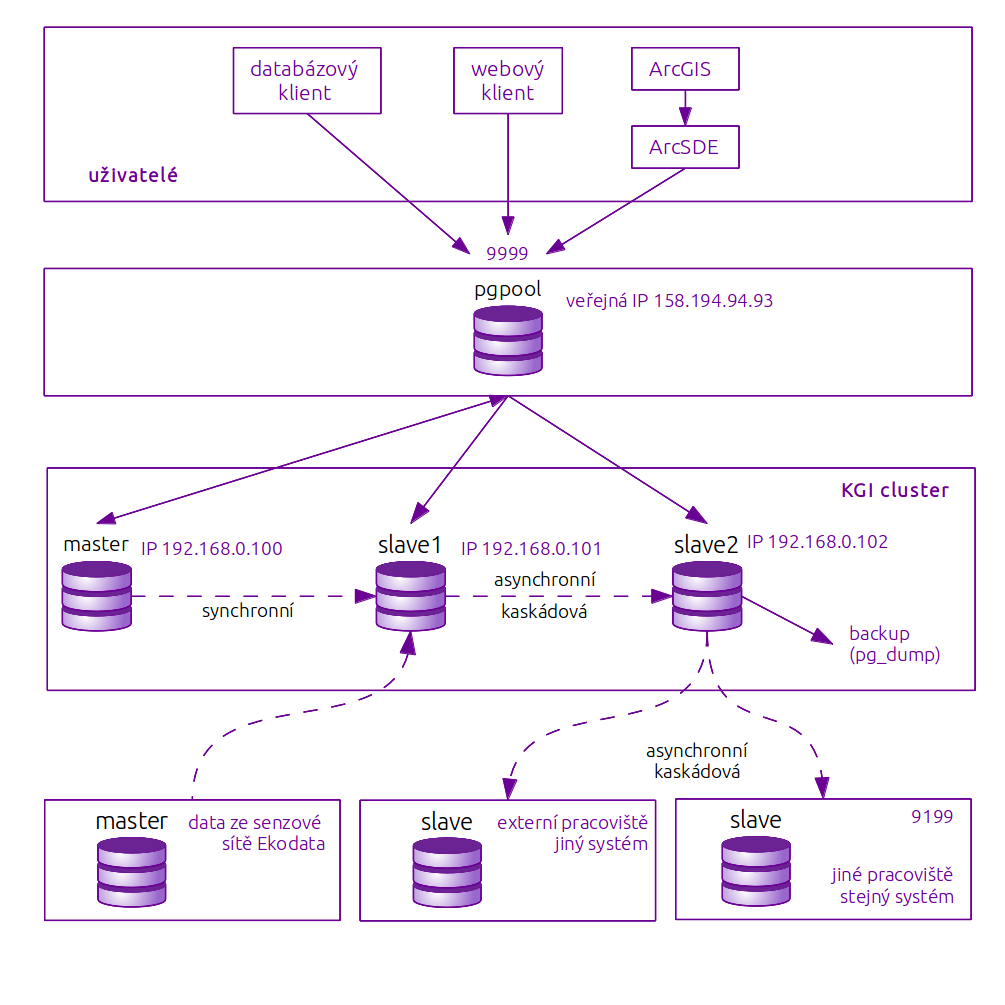
\includegraphics[width=\textwidth]{obr/schema_navrhKatedra.png}
       Srovnání multimaster a master-slave replikace
  \end{center}

Uživatelé se budou připojovat skrze nástroj pgpool, který se bude tvářit jako jediný databázový server, ke kterému se klienti přihlásí bez ohledu na typ jejich dotazu a on sám pak rozhodne, ke kterému ze serverů klienta přihlásí. Tím bude mít zároveň možnost rozložit zátěž na dostupné uzly v clusteru. Pro ještě větší efektivitu provozu databáze bude pgpool uchovávat databázová spojení a při novém dotazu využije stávajícího spojení, místo aby vytvářel spojení nové. 

Vzhledem k tomu, že klienti budou k databázovému serveru přistupovat skrze pgpool, není potřeba aby jednotlivé uzly v clusteru měly veřejnou IP adresu. Plně dostačuje, že servery poběží na lokální síti a pouze pgpool bude na serveru s veřejnou IP, čímž se zajistí, že data budou přístupná z internetu. 

Návrh počítá také s externími pracovišti, která budou často číst z databáze a~budou mít zájem o zrychlení přístupu k datům tím, že se slave server přesune na jejich pracoviště. Typ replikace se zvolí podle jejich operačního systému a jeho architektury. Pokud se bude jednat o shodný systém, jaký bude použit ve výše popsaném clusteru, pak bude možno použít asynchronní streaming replikaci, naopak pokud se bude jednat o systém jiný, bude použita Slony-I replikace. 


            \subsection{Příprava prostředí pro konfiguraci replikace}
      \label{kPriprava}
Na začátku je potřeba připravit prostředí hned s několika závislostmi. Hlavním používaným software je PostgreSQL s extenzemi PostGIS, Slony-I a pgpool. Informace o~instalacích jednotlivých komponent jsou dostupné na jejich webových stránkách. Ve Windows si stačí stáhnout pouze instalační balík pro PostgreSQL, který umožňuje instalaci databázového systému včetně všech výše zmíněných extenzí. Pro grafickou administraci databáze je doporučený, ale nepovinný, program \mbox{PgAdminIII}\footnote{http://www.pgadmin.org/}, který je taktéž multiplatformní. Většina příkazů je zde popisována skrze příkazový řádek, mají však i své ekvivalentní použití skrze grafické rozhraní.

Všechny technologie byly testovány na operačním systému Debian-based Linux, tedy některé přiklady použité v této kapitole, především pak ukázky absolutních cest k souborům, odpovídají struktuře tohoto systému. Slony-I bylo navíc vyzkoušeno také na systému Windows XP. Bylo používáno databázového systému PostgreSQL ve verzích PostgreSQL 9.1 a 9.3, Postgis verze 1.5 a 2.1, Slony-I verze 2.1 a pgpool verze 3.1 a 3.3.

Pro databázové servery byla zvolena tři datová uložiště, pro jejichž přehled \vizTabulka{tServery}. IP adresy byly pro větší názornost upraveny na rozsah běžné lokální sítě. Vzhledem k tomu, že se do databáze bude přistupovat skrze pgpoool, není potřeba, aby kterýkoli z níže vypsaných serverů, měl veřejnou IP adresu. Všechny servery běží na defaultním portu 5432, který je standardem pro PostgreSQL.

        \begin{table}[H]
          \caption[Přehled databázových serverů]{Přehled databázových serverů}
            \label{tServery}
          \begin{footnotesize}
            \begin{center}
            \begin{tabular}{lllll}
              \texttt{název serveru} & & \texttt{IP adresa} & & \texttt{port}\\
              \texttt{-------------------------} & \texttt{+} & \texttt{--------------------------} & \texttt{+} & \texttt{------------}\\
                                 \texttt{master} & \texttt{|} & \texttt{192.168.0.100} & \texttt{|} & \texttt{5432}\\
                                 \texttt{slave1} & \texttt{|} & \texttt{192.168.0.101} & \texttt{|} & \texttt{5432}\\
                                 \texttt{slave2} & \texttt{|} & \texttt{192.168.0.102} & \texttt{|} & \texttt{5432}\\
              \end{tabular}
            \end{center}
          \end{footnotesize}
        \end{table}

Aby bylo možné pracovat s databází, je nejdříve nutné chápat význam jednotlivých konfiguračních souborů a mít přehled o souborové struktuře PostgreSQL. Vzhledem k tomu, že si ji každý systém uzpůsobuje podle sebe, nezbývá než po instalaci PostgreSQL nastudovat, kde se jaký soubor nachází. Existuje tabulka \texttt{pg\_settings}, která uchovává veškeré informace o nastavení databáze. SQL příkazem volajícím tuto tabulku je možno vypsat absolutní cestu k datům (\texttt{data\_directory}) a cestu k souboru, který uchovává PID (process-ID) běžícího procesu (\texttt{external\_pid\_file}). Také popisuje tři hlavní konfigurační soubory:

\begin{itemize}
  \item \texttt{postgres.conf}, který definuje obecné nastavení databáze,
    \item \texttt{pg\_hba.conf}, který povoluje konkrétním uživatelům přístup z určitých IP adres,
    \item \texttt{pg\_ident.conf}, který slouží k mapování uživatel operačního systému na uživatele PostgreSQL \citep{ObeHsu2012}.
\end{itemize}

Příklad SQL příkazu, spuštěného na serveru master serveru, který vypíše umístění jednotlivých souborů a složek:

\begin{lstlisting}
SELECT name, setting FROM pg_settings WHERE category = 'File Locations';
\end{lstlisting}
      \begin{table}[H]
        \label{fileLocation}
        \begin{footnotesize}
          \begin{center}
            \begin{tabular}{lll}
              \texttt{name} & &\texttt{ settings}\\
                    \texttt{--------------------------------------}&\texttt{+}&\texttt{---------------------------------------------------------------------------------}\\
                      \texttt{data\_directory} & \texttt{|}&\texttt{ /var/lib/postgresql/9.1/main} \\
                  \texttt{external\_pid\_file} & \texttt{|}&\texttt{ /var/run/postgresql/9.1-main.pid} \\
                            \texttt{hba\_file} & \texttt{|}&\texttt{ /etc/postgresql/9.1/main/pg\_hba.conf}\\ 
                         \texttt{config\_file} & \texttt{|}&\texttt{ /etc/postgresql/9.1/main/postgresql.conf} \\
                          \texttt{ident\_file} & \texttt{|}&\texttt{ /etc/postgresql/9.1/main/pg\_ident.conf} \\
            \end{tabular}
          \end{center}
        \end{footnotesize}
      \end{table}

      U všech typů replikace je potřeba mít vytvořeného databázového uživatele s právem pro replikaci, pod kterým bude daný proces probíhat. Je možné vytvořit nového uživatele a nastavit mu tato práva nebo použít již existující účet \texttt{postgres}, který jako \texttt{SUPERUSER} obsahuje také práva pro replikaci. Je však potřeba mu hned na začátku změnit heslo.

Příklad změny hesla uživatele \texttt{postgres} na master serveru:
\begin{lstlisting}
ALTER ROLE postgres PASSSWORD 'kgigis';
\end{lstlisting}

Příklad vytvoření nového uživatele \texttt{replikator} s přidáním práv pro replikaci na master serveru: 
\begin{lstlisting}
CREATE ROLE replikator REPLICATION ENCRYPTED PASSWORD 'kgigis';
\end{lstlisting}

Pokud se začíná databázovým systémem, který ještě neobsahuje žádná data, je vhodné replikaci spustit ještě před přidáváním dat a to z důvodu rychlosti přenosu dat na druhý databázový server. V případě, že již databáze naplněná daty je, není problém replikaci spustit, jen je třeba počítat s delším časem kopírovaní dat a větší opatrností při konfiguraci. 

Oba typy replikace, vyžadují lehce odlišné přístupy při přípravě dat před spuštěním samotné replikace. 
Slony-I replikace vyžaduje mít předem vytvořenou strukturu databáze včetně tabulek a poté zajistit existenci totožné kopie na všech serverech v clusteru. Je možné toho dosáhnout použitím utility \texttt{pg\_dump}, která data exportuje, na master servery, a \texttt{pg\_restore}, která data importuje, na slave serveru. Tímto způsobem lze převádět jak strukturu databáze, tak data, a zároveň to umožňuje přenášet pouze vybrané části databáze. 

Příklad exportu a importu dat z databáze do databáze dat skrze:
\begin{lstlisting}[keywordstyle=\color{purpurova7},identifierstyle=\color{black},stringstyle=\color{black}]
  pg_dump > /tmp/dump.sql
  pg_restore /tmp/dump.sql
\end{lstlisting}

Streaming replikace, která funguje pouze mezi dvěmi a více databázemi běžícími na stejném systému a architektuře, vyžaduje kopii celé datové složky s daty \texttt{data\_directory}. Je mnoho způsobů, jak toho dosáhnout, například klasickým kopírováním skrze utilitu \texttt{cp}, resp. \texttt{scp} u vzdálených složek, nebo utilitou \texttt{rsync}. Kopírování dat za běhu databáze navíc vyžaduje použití příkazu \texttt{SELECT pg\_start\_backup}, který zajistí, že bude archivovat transakční log po celou dobu kopírovná, tedy až do té doby než proběhne příkaz \texttt{SELECT pg\_stop\_backup}. Tím nepřijdeme o žádné změny, které nastanou v průběhu kopírování dat.

Příklady možných způsobů zkopírování dat master serveru na repliku slave1 spuštěných z slave1:
\begin{lstlisting}
  SELECT pg_start_backup('backup', true)
\end{lstlisting}
\begin{lstlisting}[keywordstyle=\bfseries\color{purpurova7},identifierstyle=\color{black},stringstyle=\color{black}]
  scp -rv root@192.168.0.100:/var/lib/postgresql/9.1/main /var/lib/postgresql/9.1/main
  rm /var/lib/postgresql/9.1/main/postmaster.pid
\end{lstlisting}
\begin{center}
nebo 
\end{center}
\begin{lstlisting}[keywordstyle=\bfseries\color{purpurova7},identifierstyle=\color{black},stringstyle=\color{black}]
  rsync -ave ssh root@192.168.0.100:/var/lib/postgresql/9.1/main /var/lib/postgresql/9.1/main --exclude postmaster.pid
\end{lstlisting}
\begin{lstlisting}
  SELECT pg_stop_backup()
\end{lstlisting}

Stejný způsobem se provede kopie na slave2. 

Alternativou výše zmíněných nástrojů je utilita přímo určená pro zálohování dat v PostgreSQL \texttt{pg\_basebackup}. Tento příkaz mimo jiné umožňuje kopírování dat za běhu replikace bez nutnosti použití \texttt{pg\_start/stop\_backup}.

Použití \texttt{pg\_basebackup} pro vytvoření repliky:
\begin{lstlisting}[keywordstyle=\bfseries\color{purpurova7},identifierstyle=\color{black},stringstyle=\color{black}]
  pg_basebackup -D /var/lib/postgresql/9.1/main/ -U replikator -h 192.168.0.100
\end{lstlisting}

Kopírování dat je velice důležitý krok pro správný chod replikace. V případě, že se data nesprávně zkopírují, není možné replikaci zprovoznit. 

Pří kopírování celé datové struktury je vhodné zajistit jednotlivým souborům a složkám správa. Vzhledem k tomu, že databázový systém zapisuje do složky s daty \texttt{(data\_directory)}, musí mít postgres, i po zkopírování celé datové struktury na jiný server, práva pro zápis.

A v neposlední řadě je potřeba zajistit konektivitu obou, resp. všech serverů v replikačním clusteru. S tím souvisí i nutnost nastavení povolení přístupů z IP adres slave serverů, kterou je možno zajistit skrze konfigurační soubor \texttt{pg\_hba.conf}. Následující příklad ukazuje možné nastavení souboru \texttt{pg\_hba.conf} na master serveru. Povoluje uživetelům market a replication, přihlášených z dané IP adresy, přistupovat na master server a číst, resp. replikovat data.

      \begin{table}[H]
        \label{pgHba}
          \begin{center}
            \begin{tabular}{lllll}
              \texttt{\#host} & \texttt{DATABASE} & \texttt{USER} & \texttt{ADDRESS} & \texttt{METHOD} \\
                \texttt{host} & \texttt{all} & \texttt{market} & \texttt{80.188.74.1/32} & \texttt{md5} \\
       \texttt{host} & \texttt{replication} & \texttt{replication} & \texttt{80.188.74.1/32} &	\texttt{md5} \\
            \end{tabular}
          \end{center}
      \end{table}





      \subsection{Konfigurace replikace}
\label{kKonfigurace}
\subsubsection{Streaming replikace}
\label{kStreaming}
      
Jak bylo nastíněno v kapitole \odkazKapitola{kNavrh}, databázové řešení staví na
streaming replikaci a~skládá se ze tří uzlů v~clusteru - jednoho master serveru a
dvou slave serverů. Pokud je správně provedena příprava dle kapitoly
\odkazKapitola{kPriprava}, samotné nastavení replikace není nijak náročné. V
první fázi je potřeba zeditovat soubor \texttt{postgresql.conf} na master
serveru. Pro asynchonní replikaci stačí nastavit parametry:
\begin{itemize}
  \item \texttt{wal\_level}, který určuje, jaké informace mají být do transakčního
    logu (WAL) zapisovány a
  \item \texttt{max\_wal\_senders}, který nastavuje maximální počet připojených
    slave serverů.
\end{itemize}

Hodnota \texttt{wal\_level} nastavená na \texttt{hot\_stadby} zajistí, že do
transakčního logu bude zapisován takový typ informací, který poté na slave
serveru umožní dotazování. Vzhledem k tomu, že se bude na master
server připojovat pouze \texttt{slave1} a~všechny další slave servery se poté
budou připojovat k němu, hodnota \texttt{1} parametru \texttt{max\_wal\_senders}
zcela dostačuje. Je však možné hodnotu rovnou navýšit, aby se soubor v budoucnu
nemusel znovu editovat z důvodu připojení dalšího serveru.

Tyto dva parametry stačí pro nastavnení achynchronní replikace, pro nastavení
synchronní je ještě potřeba přidat parametr
\texttt{synchronous\_standby\_names}, jehož hodnota je použita při výběru slave
serverů pro synchronní replikaci (viz parametr \texttt{application\_name} u
editace souboru \texttt{recovery.conf}).

Konfigurace \texttt{postgres.conf} na master serveru:
\begin{lstlisting}
wal_level = hot_standby
max_wal_senders = 1
synchronous_standby_names = 'gis'
\end{lstlisting}

Stejně tak je potřeba konfigurovat \texttt{postgresql.conf} na slave serverech.
Hodnoty parametrů \texttt{wal\_level} a \texttt{max\_level\_sender} mohou a
nemusí zůstat stejné jako na master serveru. Pokud však má být slave připraven
zastoupit master server v případě jeho výpadku, je nutné, aby hodnoty byly
nastaveny shodně.  Na slave serveru je dále potřeba nastavit:
\begin{itemize}
  \item\texttt{hot\_standby}, který určuje, zda je na slave serveru umožněno
    dotazování a
  \item\texttt{hot\_stadby\_feedback}, který omezuje riziko přerušení
    dotazu na slave v případě kolidujících změn na master databázi.
\end{itemize}

Konfigurace \texttt{postgresql.conf} shodně na obou slave serverech:
\begin{lstlisting}
wal_level = hot_standby
max_wal_senders = 5
hot_standby = on
hot_standby_feedback = on
\end{lstlisting}

Posledním krokem je vytvoření souboru \texttt{recovery.conf} na slave serveru ve
složce s daty, který definuje parametry:
\begin{itemize}
  \item \texttt{standby\_mode}, který povoluje či zakazuje použití serveru jako
    slave a
  \item \texttt{primary\_conninfo}, který nastavuje informace o serveru, ze
    kterého budou data replikována - IP adresu serveru, port, název replikačního
    uživatele a jeho heslo a v případě synchronní replikace ještě hodnotu,
    která musí být shodná s hodnotou, která byla nastavená na master serveru v
    souboru \texttt{postgresql.conf} v~parametru
    \texttt{synchronous\_standby\_name}.
\end{itemize}

Ukázka konfigurace \texttt{recovery.conf} uloženého ve složce s daty na
\texttt{slave1}, který je připojen k master serveru a replikuje synchronně:
\begin{lstlisting}
standby_mode='on'
primary_conninfo='host=192.168.1.100 user=replikator password=kgigis application_name=gis'
\end{lstlisting}

V návrhu je počítáno s kaskádovou replikací, tedy s tím, že se \texttt{slave1}
bude připojovat k \texttt{slave2}, nikoli k master serveru. To lze nastavit
úpravou souboru \texttt{recovery.conf}, kde IP adresa parametru \texttt{host}
bude odpovídat IP adrese serveru \texttt{slave1}.

Ukázka konfigurace \texttt{recovery.conf} uloženého ve složce s daty na
\texttt{slave2}, který replikuje asynchronně a připojuje se k
\texttt{slave1}:
\begin{lstlisting}
standby_mode='on'
primary_conninfo='host=192.168.1.101 user=replikator password=kgigis'
\end{lstlisting}

To, že je replikace správně nastavená, lze zkontrolovat několika způsoby.
Připojené slave servery lze vypsat pomocí dotazu nad tabulkou
\texttt{pg\_stat\_replication}, kde poslední atribut udává, zda se jedná o
synchronní, nebo asychronní replikaci.

Výsledek dotazu spuštěného na master serveru:

\begin{lstlisting}
SELECT usename, application_name, client_addr, state, sync_state FROM pg_stat_replication;
\end{lstlisting}
\begin{table}[H]
  \label{pgHba}
  \begin{center}
    \begin{tabular}{lll}
      \texttt{-[ RECORD 1 ]----} & \texttt{+} & \texttt{--------------}\\
      \texttt{usename}           & \texttt{|} & \texttt{replikator}\\
      \texttt{application\_name} & \texttt{|} & \texttt{gis}\\
      \texttt{client\_addr}      & \texttt{|} & \texttt{192.168.1.101}\\
      \texttt{state}             & \texttt{|} & \texttt{streaming}\\
      \texttt{sync\_state}       & \texttt{|} & \texttt{sync}\\
    \end{tabular}
  \end{center}
\end{table}
Výsledek téhož dotazu spuštěného na \texttt{slave1}:
\begin{table}[H]
  \label{pgHba}
  \begin{center}
    \begin{tabular}{lll}
      \texttt{-[ RECORD 1 ]----} & \texttt{+} & \texttt{--------------}\\
      \texttt{usename}           & \texttt{|} & \texttt{replikator}\\
      \texttt{application\_name} & \texttt{|} & \texttt{walreceiver}\\
      \texttt{client\_addr}      & \texttt{|} & \texttt{192.168.1.102}\\
      \texttt{state}             & \texttt{|} & \texttt{streaming}\\
      \texttt{sync\_state}       & \texttt{|} & \texttt{async}\\
    \end{tabular}
  \end{center}
\end{table}

Stejně tak lze na slave serveru zjistit, zda skutečně replikuje z master serveru
voláním funkce \texttt{pg\_is\_in\_recovery()}:
\begin{lstlisting}
postgres=# select pg_is_in_recovery();
\end{lstlisting}
\begin{table}[H]
  \begin{center}
    \label{pgHba}
    \begin{tabular}{l}
      \texttt{pg\_is\_in\_recovery}\\
      \texttt{---------------------------------}\\
      \texttt{t}\\
      \texttt{(1 row)}\\
    \end{tabular}
  \end{center}
\end{table}

Zároveň na slave server nesmí být možné zapsat žádná data:
\begin{lstlisting}
INSERT INTO student (jmeno) VALUES('Jan Vlasovec');
\end{lstlisting}
\begin{lstlisting}[keywordstyle=\color{black},identifierstyle=\color{black},stringstyle=\color{black}]
ERROR: cannot execute INSERT in a read-only transaction
\end{lstlisting}

V případě, že master server spadne, je možné během pár minut vyměnit role a~určit
jako master jeden ze slave serverů. Lze to udělat několik způsoby, jedním z~nich
je sledování existence souboru definovaného v souboru \texttt{recovery.conf} na
kterémkoli slave serveru:
\begin{lstlisting}
trigger_file = '/tmp/trigger.txt'
\end{lstlisting}

Název souboru může být zvolen libovolně a nemusí obsahovat žádná data. Slave
server pouze hlídá jeho existenci a jen to, že se soubor objeví v dané složce,
způsobí, že slave server povýší na master. Obsah souboru mohou dále tvořit další
instrukce, které mohou ovlivnit další chod databáze.


\subsubsection{Slony-I}
      Jak už bylo zmíněno v kapitole \odkazKapitola{kSlony}, není u Slony-I možné
replikovat strukturu databáze. Výhodou však je, že lze vybrat pouze některé
tabulky k replikaci a zároveň, že se nemusí shodovat názvy databází. V tomto
ohledu tedy nabízí velkou variabilitu propojení. Jak bylo nastíněno v kapitole
\odkazKapitola{kPriprava}, nastavení replikace začíná přípravou uživatele, pod
kterým bude proces probíhat, vytvořením datové struktury a zajištění shodné
kopie dat na všech uzlech clusteru.

Pro názornost byla vytvořena databáze \texttt{studenti} a tabulky
\texttt{student} a~\texttt{rodne\_mesto}, u nichž byl nastaven \texttt{primary
key}, což je podmínkou Slony-I replikace:

\begin{lstlisting}
CREATE DATABASE studenti;
studenti=# CREATE TABLE student (id int, jmeno varchar, id_rodne_mesto int, primary key(id));
studenti=# CREATE TABLE rodne_mesto (id int, jmeno varchar, umisteni geometry, primary key(id));
\end{lstlisting}

Slony-I má vlastní konfigurační jazyk, pomocí kterého se píší skripty pro i\-ni\-ci\-a\-li\-za\-ci 
replikačního clusteru nebo pro jakoukoli změnu struktury databáze. Tyto skripty
jsou poté provedeny pomocí utility \texttt{slonik}, která se spouští
jednorázově.

Pro inicializaci clusteru skript \texttt{slonik} volá příkazy:
\begin{itemize}
  \item \texttt{cluster name} představující jedinečný název pro daný cluster,
  \item \texttt{node ival admin conninfo} definující všechny uzly v clusteru a
    parametry jejich připojení k databázi (\texttt{ival} odpovídá číslu uzlu),
  \item \texttt{init cluster}, který inicializuje cluster a nastavuje vybraný
    uzel jako master,
  \item \texttt{store node}, který vytváří další uzly,
  \item \texttt{create set} vytvářející soubor tabulek určených k replikaci,
  \item \texttt{set add table}, který přidává vždy jednu tabulku do replikačního
    setu,
  \item \texttt{store path}, který nastavuje cesty mezi jednotlivými uzly a
  \item \texttt{store listen} nastavující naslouchání jednotlivých uzlů.
\end{itemize}

Slony-I rozlišuje tři druhy serverů:
\begin{itemize}
  \item {\it origin} odpovídá master serveru, tedy jedinému uzlu, kterému je povoleno
    zapisování,
  \item {\it subscriber} je ekvivalentem slave serveru s právy čtení a
  \item {\it provider} je poskytovatel dat, může to být master server, ale při kaskádové
    replikaci také kterýkoliv ze slave serverů.
\end{itemize}

Ukázka konfiguračního skriptu pro i\-ni\-ci\-a\-li\-za\-ci replikačního clusteru nazvaného
\texttt{init\_master.txt} uloženého na master serveru:

\begin{lstlisting}[language=ruby]
# nazev clusteru
cluster name = gis_cluster;

# definice jednotlivych uzlu v clusteru
node 1 admin conninfo=$master;
node 2 admin conninfo=$slave1;
node 3 admin conninfo=$slave2;

# inicializace clusteru
init cluster (id=1, comment = 'master');
store node   (id=2, comment = 'slave1', event node=1);
store node   (id=3, comment = 'slave2', event node=1);

# vytvoreni replikacniho setu
create set (id=1, origin=1, comment='Tabulky k replikaci');
# pridani tabulek do setu
# prvni id odpovida id setu
# druhe id odpovida id uzlu masteru
# treti id je id nove pridane tabulky
set add table (set id=1, origin=1, id=1, fully qualified name = 'public.student', comment='seznam studentu');
set add table (set id=1, origin=1, id=2, fully qualified name = 'public.rodne_mesto', comment='seznam mest');

store path (server=1, client=2, conninfo=$slave1);
store path (server=1, client=3, conninfo=$slave2);
store path (server=2, client=1, conninfo=$master);
store path (server=2, client=3, conninfo=$slave2);
store path (server=3, client=1, conninfo=$master);
store path (server=3, client=2, conninfo=$slave1);

store listen (origin=1, provider=2, receiver=1);
store listen (origin=1, provider=1, receiver=2);
store listen (origin=1, provider=2, receiver=3);
\end{lstlisting}
Výskyty \texttt{\$master}, \texttt{\$slave1} a \texttt{\$slave2} je třeba nahradit
následovně:
\begin{lstlisting}
$master = 'dbname=studenti host=192.168.1.100 user=replikator password=kgigis'
$slave1 = 'dbname=studenti host=192.168.1.101 user=replikator password=kgigis'
$slave2 = 'dbname=studenti host=192.168.1.102 user=replikator password=kgigis'
\end{lstlisting}

Konfigurační skript pro i\-ni\-ci\-a\-li\-za\-ci clusteru se spustí ze složky, ve které je
uložen, příkazem \texttt{slonik} s názvem souboru:

\begin{lstlisting}
> slonik init_master.txt
\end{lstlisting}

Pomocí dalších skriptů se mohou slave servery přihlásit odběru replikačního
setu. Příklad skriptu \texttt{subscribe\_slave1.txt} pro přidání serveru do
existujícího clusteru:
%\begin{lstlisting}[identifierstyle=\color{black},stringstyle=\color{black},keywordstyle=\color{black}]
\begin{lstlisting}[language=ruby]
# nazev clusteru
cluster name = gis_cluster;

# definice jednotlivych uzlu v clusteru
node 1 admin conninfo=$master;
node 2 admin conninfo=$slave1;
node 3 admin conninfo=$slave2;

subscribe set (id=1,provider=1,receiver=2,forward=yes);
\end{lstlisting}
Výskyty \texttt{\$master}, \texttt{\$slave1} a \texttt{\$slave2} je třeba opět
nahradit, viz výše.

Spuštění skriptu \texttt{slonik} pro přidání \texttt{slave1} do clusteru:
\begin{lstlisting}
> slonik subscribe_slave1.txt
\end{lstlisting}
Stejným způsobem lze přihlásit k odběru i \texttt{slave2}.

To, že se vytvořit cluster a tabulka do něj byla přidána, lze zkontrolovat ve
výpisu, kde nově přibyly triggery, které sledují změny, které v tabulce
nastanou:

\begin{lstlisting}[language=sql]
studenti=# \d student
\end{lstlisting}

\begin{table}[H]
  \label{pgHba}
  \begin{center}
    \begin{tabular}{lllllll}
      \multicolumn{5}{c}{\texttt{Table "public.student"}} & & \\
      \texttt{Column}           & \texttt{|} & \texttt{Type}                & \texttt{|} & \texttt{Modifiers}      &    & \\
      \texttt{----------------} & \texttt{+} & \texttt{-------------------} & \texttt{+} & \texttt{--------------} &    & \\
      \texttt{id}               & \texttt{|} & \texttt{integer}             & \texttt{|} & \texttt{not null}       &    & \\
      \texttt{jmeno}            & \texttt{|} & \texttt{character varying}   & \texttt{|} &                         &    & \\
      \texttt{id\_rodne\_mesto} & \texttt{|} & \texttt{integer}             & \texttt{|} &                         & \\
      \multicolumn{7}{l}{\texttt{Indexes: "student\_pkey" PRIMARY KEY, btree (id)}} \\
      \multicolumn{7}{l}{\texttt{Triggers: \_gis\_cluster\_logtrigger AFTER INSERT OR DELETE}} \\
      \multicolumn{7}{l}{\texttt{OR UPDATE ON repl\_test FOR EACH ROW EXECUTE PROCEDURE}} \\
      \multicolumn{7}{l}{\texttt{\_is\_cluster.logtrigger('\_gis\_cluster', '1', 'k')}} \\
      \multicolumn{7}{l}{\texttt{Disabled triggers: \_gis\_cluster\_denyaccess BEFORE INSERT}} \\
      \multicolumn{7}{l}{\texttt{OR DELETE OR UPDATE ON repl\_test FOR EACH ROW EXECUTE PROCEDURE}} \\
      \multicolumn{7}{l}{\texttt{\_gis\_cluster.denyaccess('\_gis\_cluster')}} \\
    \end{tabular}
  \end{center}
\end{table}

Běh replikace je zajištěn vlastním démonem, který je možné spustit v okamžiku,
kdy je vytvořen cluster a všechny repliky jsou do něj přidány. Démon
\texttt{slon}, který je potřeba spustit na všech uzlech, v parametrech přebírá
název clusteru a hodnoty připojení daného uzlu k databázi. Je důležité, aby log
po spuštění neobsahoval žádné chyby, jinak je potřeba zkontrolovat správnost
všech příkazů konfiguračních skriptů.

Příklad spuštění démona na master serveru:
\begin{lstlisting}
> slon gis_cluster 'host=192.168.1.100 dbname=student  user=replikator'
\end{lstlisting}
Obdobně je démon spuštěn i na obou slave serverech:
\begin{lstlisting}
> slon gis_cluster 'host=192.168.1.101 dbname=student  user=replikator'
> slon gis_cluster 'host=192.168.1.102 dbname=student  user=replikator'
\end{lstlisting}

Stějně jako u streaming replikace, lze zkontrolovat, že replikace běží správně,
pokusem o přidání nového záznamu na slave server. Pokud nepovolí přidání a
vypíše následující chybu, je replikace nastavena správně.

\begin{lstlisting}
studenti=# INSERT INTO student (jmeno) VALUES ('Josef Kraus');
\end{lstlisting}
\begin{lstlisting}[identifierstyle=\color{black},stringstyle=\color{black},keywordstyle=\color{black}]
ERROR:  Slony-I: Table student is replicated and cannot be modified on a subscriber node - role=0
\end{lstlisting}

Přidání další tabulky či jakákoli jiná změna struktury databáze probíhá v
několika krocích. Nejdříve je potřeba vytvořit soubor, který bude obsahovat SQL
příkaz provádějící zvolenou změnu databáze. Poté se spustí program
\texttt{slonik}, který vykoná SQL příkaz na všech uzlech clusteru.

Příklad souboru \texttt{createTable.sql}:

\begin{lstlisting}
CREATE TABLE predmet (id int, jmeno varchar, primary  key(id));
\end{lstlisting}

Příklad skriptu \texttt{ddlZmena.txt}, který umožní přidání tabulky za chodu
replikace:

%\begin{lstlisting}[identifierstyle=\color{black},stringstyle=\color{black},keywordstyle=\color{black}]
\begin{lstlisting}[language=ruby]
# nazev clusteru
cluster name = gis_cluster;

# definice jednotlivych uzlu v clusteru
node 1 admin conninfo=$master;
node 2 admin conninfo=$slave1;
node 3 admin conninfo=$slave2;

execute script (
SET ID = 1,
filename = '/tmp/createTable.sql',
event node = 1
);
\end{lstlisting}
Výskyty \texttt{\$master}, \texttt{\$slave1} a \texttt{\$slave2} je třeba opět
nahradit, viz výše.


Spuštění programu \texttt{slonik}, který vykoná daný SQL příkaz na všech uzlech:

\begin{lstlisting}
> slonik ddlZmena.txt
\end{lstlisting}
\begin{lstlisting}[identifierstyle=\color{black},stringstyle=\color{black},keywordstyle=\color{black}]
DDL script consisting of 2 SQL statements
DDL Statement 0: (0,67) [ CREATE TABLE predmety (id int, nazev varchar, primary key(id));]
slony_ddl.txt:6: NOTICE:  CREATE TABLE / PRIMARY KEY will create implicit index "predmety_pkey" for table "predmety"
DDL Statement 1: (67,69) [ ]
Submit DDL Event to subscribers...
\end{lstlisting}

Podrobný výpis informuje, že se změnilo schéma databáze. Posledním řádkem
potvrzuje, že se schéma zapsalo také na slave servery. Takto se tabulka přidá do
databáze, nikoliv však do replikačního setu. K tomu je potřeba vytvořit
další slonik skript.

Příklad skriptu \texttt{add\_to\_set.txt} pro přidání tabulky do replikačního
setu:

%\begin{lstlisting}[identifierstyle=\color{black},stringstyle=\color{black},keywordstyle=\color{black}]
\begin{lstlisting}[language=ruby]
# nazev clusteru
cluster name = gis_cluster;

# definice jednotlivych uzlu v clusteru
node 1 admin conninfo=$master;
node 2 admin conninfo=$slave1;
node 3 admin conninfo=$slave2;

# definice noveho setu (id 2)
create set (id=2, origin=1, comment='Dalsi tabulky k replikaci');

# pridani nove vytvorene tabulky
set add table (set id=2, origin=1, id=3, fully qualified name = 'public.predmet', comment='seznam predmetu');

# pridani noveho setu id=2
subscribe set (id=2, provider=1, receiver=2);

# spojeni setu id2 se setem id1
merge set(id=2, add id=1, origin=1);
\end{lstlisting}
Výskyty \texttt{\$master}, \texttt{\$slave1} a \texttt{\$slave2} je třeba opět
nahradit, viz výše.

Spuštění skriptu \texttt{slonik}, který příkazy vykoná:

\begin{lstlisting}
> slonik add_to_set.txt
\end{lstlisting}

Podobně je lze také smazat tabulku příkazem \texttt{drop set}. 



      \subsection{Rozložení zátěže mezi replikační servery}

Doposud je samotné replikační rešení nastaveno tak, že se uživatelé musí přihlašovat vždy ke konkrétnímu serveru v clusteru. To není úplně vhodné řešení, protože v případě, že se na jeden uzel, například v rámci cvičení, připojí velký počet klientů, může se stát, že se daný server přetíží, zatímco druhý slave server nezaznamená žádnou zátěž. Zároveň by pro plynulý běh databázového clusteru bylo vhodné, aby se uživatelé s dotazy SELECT, připojovali pouze na slave servery, zatímco příkazy, které modifikují data (CREATE, INSERT, DELETE), byly vykonány na master serveru. 

Oba výše diskutované problémy řeší nástroj \texttt{pgpool}, který bude použit v módu \texttt{master/slave} a který zajistí, že se všechny příkazy provádějící změnu v databázi pošlou na master server a ostatní dotazy budou rozloženy mezi slave servery. Dotazy na master server bohužel nemohou být rozloženy, protože v replikačním clusteru smí být vždy jen jeden server s právem pro zapis. Toto řešení zajistí také zvýšení dostupnosti dat, protože tím, že bude mít uživatel přístup ke všem serverům místo pouze jednoho, nebude vůbec omezen výpadkem kteréholi uzlů na straně serveru.

    Konfigurace pgpool se skládá ze tří hlavních souborů:
\begin{itemize}
  \item \texttt{pcp.conf}, který nastavuje přístupové jméno a heslo pro administrátora pgpool, 
  \item \texttt{pool\_hba.conf}, který povoluje přístupy k pgpool pro konkrétní uživatele, soubor je podobný jako pg\_hba.conf v PostgreSQL a 
  \item \texttt{pgpool.conf}, který zajišťuje obecné nastavení. 
\end{itemize}

Nejdříve je potřeba nastavit heslo pro administrátora, který bude moct měnit nastavení a sledovat statistiky. Heslo lze vytvořit pomocí ulitity \texttt{pg\_md5}, která vrátí zadané zašifrované heslo, které je poté potřeba zkopírovat do souboru \texttt{pcp.conf} a doplnit jej o uživatelské jméno.

Příklad zašifrování hesla \texttt{kgigis} pomocí \texttt{pg\_md5} s vypsaným výsledkem:
%\begin{lstlisting}[identifierstyle=\color{black},stringstyle=\color{black},keywordstyle=\color{black}]
\begin{lstlisting}[language=ruby,morekeywords={pg_md5}]
pg_md5 kgigis
eea831dcf9dc85ace5836024f3a253e7
\end{lstlisting}

Přidání přihlašovacích údajů pro administrátora do souboru \texttt{pcp.conf}:
%\begin{lstlisting}[identifierstyle=\color{black},stringstyle=\color{black},keywordstyle=\color{black}]
\begin{lstlisting}[language=ruby]
#username:[password encrypted in md5]
kgi:eea831dcf9dc85ace5836024f3a253e7
\end{lstlisting}


Zvolený master/slave mód počítá s již nastavenou replikací a podporuje jak streaming replikaci, tak Slony-I. Pro usnadnění konfigurace pgpool poskytuje příklady všech konfiguračních souborů včetně různých typů nastavení. Pro master/slave mód jsou připraveny hned dva příkladové soubory, \texttt{pgpool.conf.sample-master-slave} pro Slony-I a \texttt{pgpool.conf.sample-stream} pro streaming replikaci. V případě použití této šablony, je nejdříve potřeba ji přesunout do složky s konfiguračními soubory a poté přejmenovat na \texttt{pgpool.conf}. Šablona zajistí základní konfiguraci pro mód master/slave a streaming replikaci, nastaví parametry:
\begin{itemize}
\item \texttt{replication\_mode}, který povoluje replikaci, výchozí hodnota je off, 
\item \texttt{load\_balance\_mode}, který umožňuje rozložení zátěže, východí hodnota je off
\item \texttt{master\_slave\_mode}, který povoluje propojení k master a slave serverů, 
\item \texttt{master\_slave\_sub\_mode}, který nastavuje hodnotu na 'stream’ v případě streaming replikace a ‘slony' v případě Slony-I, 
\item \texttt{sr\_check\_period = 10}, který nastavuje jak často má systém zkontrolovat pozici v XLOGu, aby zjistil, jestli je zpoždění příliš vysoké, či nikoli, 
\item \texttt{delay\_threshold}, která definuje maximální možné zpoždění slave za master serverem, menší zpozdeni je možno nastavit v případě, ze je potřeba, aby replikace proběhla velice rychle (hodnota je určena v bytech) a 
\end{itemize}

Část konfiguračního souboru \texttt{pgpool.cong} s výpisem důležitějších parametrů a jejich hodnot:
%\begin{lstlisting}[identifierstyle=\color{black},stringstyle=\color{black},keywordstyle=\color{black}]
\begin{lstlisting}[language=ruby]
replication_mode = off	
load_balance_mode = on	
master_slave_mode = on	
master_slave_sub_mode = 'stream'
sr_check_period = 10
log_standby_delay = 'if_over_threshold'
delay_threshold = 10000000 
\end{lstlisting}

Další část konfiguračního souboru přidává konkrétní uzly, ke kterým bude po spuštění pgpool možno přistupovat právě přes pgpool. Pro uživatele se v podstatě nic nezmění, k databázi se připojí stejně, jako by se přihlašovali přímo, s jediným rozdílem, že použijí port definovaný v tom souboru parametrem \texttt{port}. Číslo za parametrem začínájícím \texttt{backend} vždy značí číslo daného nodu přidaného do pgpool. V tomto případě jsou přidány tři uzly, který byla přiřazena čísla 0 pro master, 1 pro slave1, 2 pro slave2. Parametr: 
\begin{itemize}
\item \texttt{listen\_addresses} definuje IP adresy, na kterých pgpool naslouchá, 
\item \texttt{port} definuje port, kterým se uživatelé budou přihlašovat k databázovému clusteru (místo nejčastnějšího 5432), 
\item \texttt{pcp\_port} určuje port, kterým se bude přihlašovat administrátor, 
\item \texttt{backend\_hostname} nastavuje hosta nebo IP adresu daného uzlu, 
\item \texttt{backend\_port0} určuje port, na kterém naslouchá daný uzel, 
\item \texttt{backend\_weight} umožňuje zvýšit danému uzlu zátěž, čím vyšší číslo, tím více datazů bude směřováno na tento uzel místo, 
\item \texttt{backend\_data\_directory} určuje, kde jsou uložená data daného uzlu a 
\item \texttt{backend\_flag} povoluje nebo zakazuje daný uzel použít jako master v případě výpadku master servera.
\end{itemize}

Čast konfigurace souboru \texttt{pgpool.conf}, která nastavuje jednotlivé uzly:
\begin{lstlisting}[language=ruby]
listen_addresses = '*'
port = 9999 		
pcp_port = 9898 	

# node 0 - master server
backend_hostname0 = '192.168.1.100' 			
backend_port0 = 5432 					
backend_weight0 = 1					
backend_data_directory0 ='/var/lib/postgresql/9.3/main'
backend_flag0 = 'ALLOW_TO_FAILOVER'	      

# node1 - slave1
backend_hostname1 = '192.168.1.101'
backend_port1 = 5432
backend_weight1 = 1
backend_data_directory1 = '/var/lib/postgresql/9.1/main'
backend_flag1 = 'ALLOW_TO_FAILOVER'

# node2 - slave2
backend_hostname2 = '192.168.1.102'
backend_port2 = 5432
backend_weight2 = 1
backend_data_directory2 = '/var/lib/postgresql/9.1/main'
backend_flag2 = 'ALLOW_TO_FAILOVER'
\end{lstlisting}

Pro správný běh pgpool je potřeba, aby slave server, který má hodnotu \texttt{backend\_flag2 'ALLOW\_TO\_FAILOVER'} měl v souboru \texttt{recovery.conf} přidán parametr \texttt{trigger\_file}, již popisovaný v kapitole \odkazKapitola{kStreaming}.

Než dojde k samotnému spuštění pgpool, je možno zkontrolovat, zda jsou všechny uzly přidány a běží, tak jak mají. Lze použít utilitu \texttt{pcp\_node\_count}, který vypíše počet aktuálně přidaných uzlů. Zadání dále vyžaduje difinici parametrů v pořadí:
 \begin{itemize}
\item \texttt{timeout}, který učí maximální čas, po který se má snažit o vykonání příkazu v sekundách,
\item \texttt{hostname}, který definuje pgpool IP,
\item \texttt{port} definovaný pro administrátora,
\item \texttt{username} odpovídá uživatelskému jménu zadanému v pcp.conf a 
\item \texttt{password} odpovídá heslu definovanámu v pcp.conf a

\end{itemize}

Spuštění nástroje \texttt{pcp\_node\_count} s maximálním časem provedení 30 sekund, pgpool běžícím na localhostu, portem 9898, uživatel kgi a heslem kgigis:
\begin{lstlisting}[language=ruby]
pcp_node_count 30 localhost 9898 kgi kgigis
3
\end{lstlisting}

Obdobně lze získlad informace o konkrétních uzlech utilitou \texttt{pcp\_node\_info}, která navíc přidává parametr \texttt{nodeID}, který odpovídá ID uzlu, o kterém chceme získat informace.

Spuštění nástroje \texttt{pcp\_node\_info} pro uzly 0, 1 a 2 s maximálním časem provedení 30 sekund, pgpool běžícím na IP adrese 127.0.0.1, portem 9898, uživatel kgi a heslem kgigis:
\begin{lstlisting}[language=ruby]
pcp_node_info 30 192.169.1.100 9898 kgi kgigis 0
192.168.1.100 5432 1 0.333333
pcp_node_info 30 192.169.1.101 9898 kgi kgigis 1
192.168.1.101 5432 1 0.333333
pcp_node_info 30 192.169.1.102 9898 kgi kgigis 2
192.168.1.102 5432 1 0.333333
\end{lstlisting}

pgpool nabízí ještě další nástroje, pomocí který lze získat informace o nastavení pgpool (\texttt{pcp\_pool\_info} nebo \texttt{pcp\_promote\_node} pro změnu uzlů z master na slave a opačně\footnote{kompletní seznam nástrojů pgpool na \url{http://www.pgpool.net/docs/latest/pgpool-en.html\#pcp\_command}}. 

Posledním krokem je spuštění démona pgpool. 
/etc/init.d/pgpool2 start|status|stop

      \subsection{Připojení databáze skrze ArcSDE}

Pro možnost připojení dat z databázového serveru PostgreSQL k produktům ArcGIS,
je potřeba nainstalovat PostgreSQL doplněný o knihovny ArcSDE. Instalační balík
lze stáhnout na {\it Esri Customer Care Portal
\footnote{https://customers.esri.com/}} a nainstalovat jej dle návodů dostupných na
{\it ArcGIS Resource Center
\footnote{http://resources.arcgis.com/en/help/main/10.1/index.html\#//002p000000t4000000}}.
U výběru verzí je nutné zajistit kompatibilitu verzí jednotlivých programů, viz kapitola \ref{kArcSDE}.

Po instalaci a konfiguraci PostgreSQL i knihoven ArcSDE je možno vytvořit
prostorovou databázi pomocí nástroje \texttt{Create Enterprise Geodatabase}
spuštěným na ArcGIS for Desktop (Standard nebo Advanced) nebo pomocí Python
skriptu. Takto lze existující databázi přidat schéma \texttt{sde}, které nese prostorové
funkce, indexy a datové typy, nebo vytvořit novou databázi s tímto schématem
\odkazObrazek{o}. ArcGIS produkty lze vždy připojit pouze k tabulkám, které jsou
uloženy ve schématu \texttt{sde}. 

  \begin{figure}[H]
    \centering
    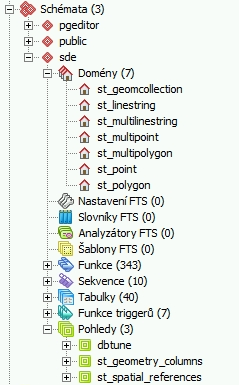
\includegraphics[scale=0.6]{../../../grafy/obr/sde_schema.png}
    \caption{Příklad struktury vytvořeného schématu sde}{Příklad struktury vytvořeného schématu \texttt{sde}}
          \label{o}
  \end{figure}

K databázi je poté možno se připojit obdobně jak u PostgreSQL. Přihlašovací
okno lze sputit pomocí ArcCatalogu, výběru Database Connections a volby
Database Connection, která otevře okno s možností zadání
přihlašovacích údajů \odkazObrazek{connect}. Pouze u první volby \texttt{Database Platform} je třeba vybrat jako databázového systém PostgreSQL. 

  \begin{figure}[H]
    \centering
    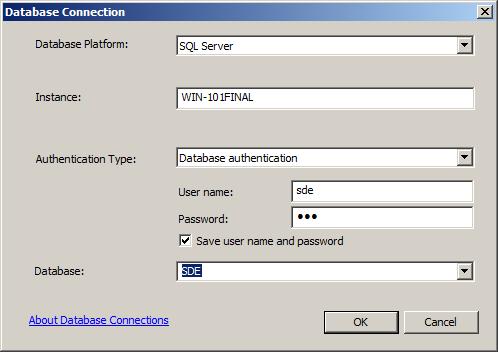
\includegraphics[scale=0.5]{../../../grafy/obr/conectScreen.png}
    \caption {Ukázka připojení databáze skrze ArcSDE}
          \label{connect}
  \end{figure}


      \subsection{Testování výkonu}
Před spuštěním databází to reálného provozu je vhodné provést optimalizaci nastavení nejen replikace, ale celého databází řešení. To zahrnuje jak konkrétní nastavení konfiguračních souborů, ale také zahrnutí všech atributů, jako výkonost serverů, na kterých databáze běží, rychlost sítě, způsobu užívání databáze, počet uživatelů atd. 

V rámci pozorování chování databáze bylo zjištěno, že data i většího rozsahu jsou přeneseny v řádech vteřin. Je však nutno zohlednit, že všechny tři uzly běži po vnitřní síti, což rychlost přenosu zvyšuje. Zároveň nebyl zaznamenán případ, kdyby se přenesla pouze část dat nebo byla některá přenesená data chybná. 

Při použití pgpool je možno testovat rozdíl počtu transakcí za sekundu v případě připojení pouze na master, resp. slave server a na pgpool. V ideální případě by měl pgpool znásobit počet transakcí o třetinu. Tím, že se zvýší počet transakcí za sekundu, je možno zjistit, že pgpool efektivně rozkládá dotazy mezi jednotlivé uzly. Je třeba zohlednit, že pgpool nějakou dobu vyhodnocuje příkaz, než jej přepošle dál. To může proces mírně zpomalit, pak záleží na tom, jak velké dotazy jsou do něj posílány. 
Testování je vždy potřeba testovat až na hotovém řešení s ohledem na konkrétní nastavení, zohlednit je potřeba i typy operací, které jdou v databázi vykonávány, např. jaké příkazy provádí ArcGIS server.
Dá se vycházet z předpokladů, že při synchronní i asynchronní replikaci by nemělo docházet ke zpomalení přenosu transakcí při čtení z databáze a stejně tak u asynchronní replikace při zápisu na master. V případě zápisu do databáze může mít vliv synchronní replikace, která čeká, až je dotaz zapsán na slave, synchronní možné zpomalení vlivem latence sítě. 

Pro testování výkonu existuje několik nástrojů, například pgbench. 


    %------------------------------------------------------------------------- DISKUZE
    \newpage
    \section{DISKUZE}
      \label{kDiskuze}
Jedním z požadavků pro výběr databázového systému bylo rozšířené používání v~oblasti
geoinformatiky a~zároveň podpora ArcGIS produkty. Z tohoto důvodu nemohl být použit
databázový server MySQL, který je sice v oblasti GIS používaný, není však
podporovaný produkty Arc\-GIS. Opačný problém je řešen u MS SQL Serveru, který je
doposud na katedře používán a který je podporován ArcGIS produkty, není však
tak široce používaný v oblasti geoinformatiky. Jeho rozšíření o prostorová data
totiž například nepoužívá nástroje pro transformaci dat, které jsou v~PostgreSQL řešeny knihovnou OGR. 

U výběru replikačního nástroje se vycházelo z nativního řešení pro PostgreSQL, který
podporuje pouze master-slave replikaci. Při velkém počtu editací by přicházelo v~úvahu použití multimaster replikace, pro kterou je však třeba použít
některého z~externích nástrojů a jejíž konfigurace je složitější. 

Replikační řešení je navrženo tak, že je zcela nezávislé na technologii ArcSDE.
ArcSDE je v tom řešení pouze prostředníkem pro připojení databáze k ArcGIS
produktům. Replikaci je tedy možno nastavit bez ohledu na ArcSDE, přičemž po přidání schématu
\texttt{sde} do databáze, lze replikovat také tabulky toho schématu. 

Jak už bylo několikrát zmíněno, pro fungování celého řešení, tedy včetně
připojení databáze k ArcGIS produktům, je potřeba zajistit kompatibilitu jednotlivých verzí.
Tento fakt byl zjištěn příliš pozdě, proto se jej při vytváření testovacího prostředí nepodařilo dodržet.
Přesto byly všechny programy nastudovány, otestovány a podrobně v této práci zdokumentovány,
při příštím vytváření databázového clusteru by tedy nemělo dojít k výše zmíněným problémům.

K databázi přes ArcSDE lze připojit jak verze ArcGIS for
Desktop, tak ArcGIS for Server. Verzi ArcGIS Online nelze připojit k databázi
přímo, ale pouze přes vrstvu publikovanou ArcSDE. 

Pro efektivní fungování databáze by ještě předtím než bude
datázové řešení spuštěno do plného provozu, měla být provedena optimalizace nastavení
databázového systému a testování zátěže. Optimalizace by měla zohlednit počty uživatelů
přistupujících k databázi stejně tak jako náročnost jejich dotazů. V rámci
optimalizace je možno testovat zátěž pomocí pgbench, důvody pro jeho použití
byly nastíněny v kapitole \odkazKapitola{kpgbench}, nebo jiného dostupného
nástoje. Jedná se však o složitý problém, který vyžaduje bohaté zkušenosti s
provozem databázového systému a široké znalosti nejen v oblasti databází, ale
také počítačové techniky.  

Nástroj pgpool, který v návrhu zajišťuje rozkládání dotazů mezi servery v
clusteru, nesleduje, jaké je aktuální vytížení serveru jinými procesy. Pro řízení
load ba\-la\-ncing používá náhodného rozdělování dotazů mezi jednotlivé uzly. 
Pokud už na serveru běží jiné služby (např. geoportál), které nesmí být ve svém
provozu omezeny, je možno zátěž, kterou pgpool směřuje na jednotlivé slave
servery, ovlivnit parametrem \texttt{backend\_weight}. Jeho hodnotou lze proporčně
nastavit zátěž jednotlivých uzlů, jak již bylo ukázáno v kapitole
\ref{kRozlozeni}. Takto lze například snížit počet dotazů, které jsou
směřovány na server, zatížený jinými službami.



    %------------------------------------------------------------------------- ZÁVĚR
    \newpage
    \section{ZÁVĚR}
      \label{kZaver}
Tato práce hodnotí možnosti dostupných replikačních řešení a na základě toho navrhuje databázové řešení s ohledem na možnosti a požadavky katedry. V rešerší části byly vymezeny pojmy synchronizace, replikace a související pojem verzování a~popsána replikace včetně variant synchronní, asynchronní, jednosměrné, obou\-smě\-rné, kaskádové, logické i fyzické. Byly rozebrány požadavky na databázové ukládání dat jednotlivých produktů ArcGIS a byla podrobně popsána technologie ArcSDE, která se v ArcGIS produktech používá pro připojení k databázi.

Na základě rešerše byl vybrán databázový systém PostgreSQL, který je možno použít v kombinaci s produkty ArcGIS, což bylo jedním z hlavních požadavků pro výběr databázového systému. Byl sestaven návrh databázového řešení, který zohledňuje všechny požadavky katedry a možnosti daných technologií. Bylo vytvořeno testovací prostředí na serveru poskytnutém katedrou, na němž byly dané procesy otestovány. Na základě toho byl pak sepsán podrobný popis toho, jak nastavit replikaci ve variantě streaming a Slony-I. Návrh zahrnuje také možnost použití nástroje pgpool pro rozložení zátěže mezi servery v databázovém clusteru.

Návrh databázového řešení slibuje zvyšení interoperability, usnadnění sdílení dat a~dodržování licenčních podmínek, zajištění vysoké dostupnosti a aktuálnosti dat. Studenti navíc budou mít možnost vyzkoušet si pokročilou práci s databází, která je může lépe připravit na budoucí zaměstání.


    %------------------------------------------------------------------------- LITERATURA
    \makeBibliography{literatura}

    %------------------------------------------------------------------------- SUMMARY
    \begin{summary}
      The main goal of this thesis is to evaluate options of replication
solutions which are available and based on this research design a database solution which
considers possibilities and requirements of the Department of
Geoinformatics. In the theoretical part terms replication,
synchronization and versioning are defined including description of
synchronous, asynchronous, master-slave, multimaster, cascade, logical and
physical replication. The requirements of ArcGIS products for storage of data
in database were considered and ArcSDE Technology which is used by ArcGIS products
for database storage of spatial data was described. 

Based on the research database management system PostgreSQL was chosen because
it is supported by ArcGIS products. The design of the database solution was
created based on all requirements and the main processes were tested. Based on
that a manual of the proposed replication solution setup was written. Two 
replication options were tested - PostgreSQL native streaming replication
and replication using PostgreSQL extension Slony-I. The design includes a description of usage of pgpool utility used for
load-balancing. 






    \end{summary}

    %------------------------------------------------------------------------- PŘÍLOHY
    \newpage
    \addcontentsline{toc}{section}{PŘÍLOHY}
    \vspace*{180pt}
    \begin{center}
    \section*{PŘÍLOHY}
    \end{center}
    \vspace*{\fill}

    \newpage
    \begin{prilohy}
      \textbf{Volné přílohy}

      Příloha 1 CD \newline
      \newline
      \textbf{Popis sktruktury CD}

        Adresáře a soubory:

        - \texttt{web\slash} - webové stránky jako doplněk k diplomové práci

        - \texttt{Solanska\_DP.pdf} - text diplomové práce

      \vspace*{\fill}
  \end{prilohy}

  \end{document}
